\documentclass[11pt]{cernrep}
\usepackage{graphicx,epsfig}
\bibliographystyle{lesHouches}


% Packages needed for this section
\usepackage{amsmath}
\usepackage{hepunits}
\usepackage[caption=false]{subfig}
\usepackage[utf8]{inputenc}

% Comments to be commented out when done
%\usepackage{color}
%\definecolor{darkgreen}{rgb}{0,0.5,0}
%\newcommand{\jdt}[1]{\textbf{\textcolor{darkgreen}{(#1 --jdt)}}}
%\definecolor{darkblue}{rgb}{0,0,0.5}
%\newcommand{\gs}[1]{\textbf{\textcolor{darkblue}{(#1 --gs)}}}

\begin{document}

\section{SYSTEMATICS OF QUARK/GLUON TAGGING\protect\footnote{Section coordinators: Gregory Soyez and Jesse Thaler}$^{,}$\protect\footnote{Contributing authors: Marat Freytsis, Philippe Gras, Deepak Kar, Leif L\"onnblad, Simon Pl\"atzer, Andrzej Siodmok, Peter Skands, and Davison Soper}$^{,}$\protect\footnote{Additional input: Samuel Bein, Andy Buckley, Jon Butterworth, Mario Campanelli, Andrew Larkoski, Peter Loch, Ben Nachman, Zoltan Nagy, Chris Pollard, Salvatore Rappoccio, Gavin Salam, Alexander Schmidt, Frank Tackmann, and Wouter Waalewijn}}

By measuring the substructure of a jet, one can assign it a ``quark'' or ``gluon'' tag.  In the eikonal limit, quark/gluon discrimination is determined solely by the color factor of the initiating parton ($C_F$ versus $C_A$).  In this section, we confront the challenges faced when going beyond this leading-order understanding, using parton shower generators to assess the impact of higher-order perturbative and nonperturbative physics.  Working in the idealized context of electron-positron collisions, where one can define a proxy for quark and gluon jets based on the Lorentz structure of the production vertex, we find a fascinating interplay between perturbative shower effects and nonperturbative hadronization effects.

\subsection{Overview}
\label{quarkgluon_sec:overview}

Jets are a robust tool for studying short-distance collisions involving quarks and gluons.  With a suitable jet definition, one can connect jet measurements made on clusters of hadrons to perturbative calculations made on clusters of partons.  More ambitiously, one can try to tag jets with a suitably-defined flavor label, thereby enhancing the fraction of, say, quark-tagged jets over gluon-tagged jets.  This is relevant for searches for physics beyond the standard model, where signals of interest are often dominated by quarks while the corresponding backgrounds are dominated by gluons.  A wide variety of quark/gluon discriminants have been proposed \cite{Gallicchio:2011xq,Gallicchio:2012ez,Krohn:2012fg,Pandolfi:1480598,Chatrchyan:2012sn,Larkoski:2013eya,Larkoski:2014pca,Bhattacherjee:2015psa}, and there is a growing catalog of quark/gluon studies at the Large Hadron Collider (LHC) \cite{Aad:2014gea,Aad:2014bia,Khachatryan:2014dea,Aad:2015owa,Khachatryan:2015bnx,Aad:2016oit}.

In order to achieve robust quark/gluon tagging, though, one needs theoretical and experimental control over quark/gluon radiation patterns.  At the level of eikonal partons, a quark radiates proportional to its $C_F = 4/3$ color factor while a gluon radiates proportional to $C_A = 3$.  In this section, we demonstrate that quark/gluon discrimination performance is highly sensitive to subleading perturbative effects beyond the eikonal limit, such as $g \to q \overline{q}$ splittings and color coherence, as well as to nonperturbative effects such as color reconnection and hadronization.   While these effects are modeled (to differing degrees) in parton shower generators, they are relatively unconstrained by existing collider measurements, especially in the gluon channel.  The goal of this section is to highlight these uncertainties, which then suggests a set of future LHC measurements that will improve the modeling of jets in general and quark/gluon tagging in particular.

A common misconception about quark/gluon tagging is that it is an intrinsically ill-defined problem.  Of course, quark and gluon partons carry color while jets are composed of color-singlet hadrons, so the labels ``quark'' and ``gluon'' are fundamentally ambiguous. 
But this is philosophically no different from the fact that a ``jet'' is fundamentally ambiguous and one must therefore always specify a concrete jet finding procedure.  As discussed in Sec.~\ref{quarkgluon_sec:def}, one can indeed create a well-defined quark/gluon tagging procedure based unambiguous hadron-level measurements.  In this way, even if what one means by ``quark'' or ``gluon'' is based on a naive or ambiguous concept (like Born-level cross sections or eikonal limits), quark/gluon discrimination is still a well-defined technique for enhancing desired signals over unwanted backgrounds.
  
There are a wide range of possible quark/gluon discriminants and a similarly large range of ways to quantify discrimination power.  As a concrete set of discriminants, we consider the generalized angularities $\lambda_\beta^\kappa$ \cite{Larkoski:2014pca} (see also \cite{Berger:2003iw,Almeida:2008yp,Ellis:2010rwa,Larkoski:2014uqa}),
\begin{equation}
\label{quarkgluon_eq:genang_intro}
\lambda^{\kappa}_{\beta} = \sum_{i \in \text{jet}} z_i^\kappa \theta_i^\beta,
\end{equation}
with the notation to be explained in Sec.~\ref{quarkgluon_sec:genang}.  We consider five different $(\kappa, \beta)$ working points, which roughly map onto five variables in common use in the literature:
\begin{equation}
\begin{array}{ccccc}
(0,0) & (2,0) & (1,0.5) & (1,1) & (1,2) \\
\text{multiplicity} &  p_T^D &  \text{LHA} & \text{width} & \text{mass}
\end{array}
\end{equation}
Here, multiplicity is the hadron multiplicity within the
jet, $p_T^D$ was defined in
Refs.~\cite{Pandolfi:1480598,Chatrchyan:2012sn}, LHA refers to the
``Les Houches Angularity'' (named after the venue of this workshop),
width is closely related to jet broadening
\cite{Catani:1992jc,Rakow:1981qn,Ellis:1986ig}, and mass is closely
related to jet thrust \cite{Farhi:1977sg}.  To quantify discrimination
performance, we focus on classifier separation (a default output of
TMVA \cite{2007physics...3039H}):
\begin{equation}
\label{quarkgluon_eq:deltadef_intro}
\Delta =  \frac{1}{2} \int \text{d} \lambda \, \frac{\bigl(p_q(\lambda) - p_g(\lambda)\bigr)^2}{p_q(\lambda) + p_g(\lambda)},
\end{equation}
where $p_q$ ($p_g$) is the probability distribution for $\lambda$ in a generated quark jet (gluon jet) sample.  This and other potential performance metrics are discussed in
Sec.~\ref{quarkgluon_sec:classsep}.

We begin our parton shower generator predictions for quark/gluon discrimination in Sec.~\ref{quarkgluon_sec:ee}, using an idealized setup with $e^+e^-$ collisions.  Here, we can use the following processes as proxies for quark and gluon jets:
\begin{align}
\text{``quark jets''}: \quad & e^+e^- \to (\gamma/Z)^* \to u \overline{u}, \\
\text{``gluon jets''}: \quad & e^+e^- \to h^* \to g g,
\end{align}
where $h$ is the Higgs boson.  These processes are physically
distinguishable by the quantum numbers of the associated color singlet
production operator, giving a way to define truth-level quarks and
gluons labels without reference to the final state.\footnote{Of course, the quantum numbers of the color singlet operator are not measurable event by event.  The idea here is to have a fundamental definition of ``quark'' and ``gluon'' that does not reference QCD partons directly.}  We
compare six different parton shower generators both before
hadronization (``parton level'') and after hadronization (``hadron
level''):
\begin{itemize}
\item \textsc{Pythia 8.205} \cite{Sjostrand:2006za,Sjostrand:2014zea},
\item \textsc{Herwig++ 2.7.1} \cite{Bahr:2008pv,Bellm:2013hwb},
\item \textsc{Sherpa 2.1.1} \cite{Gleisberg:2008ta},
\item \textsc{Vincia 1.201} \cite{Giele:2013ema},
\item \textsc{Deductor 1.0.2} \cite{Nagy:2014mqa} (with hadronization performed by \textsc{Pythia 8.212}),\footnote{Note that this
\textsc{Deductor} plus \textsc{Pythia} combination has not yet been tuned to data.}
\item \textsc{Ariadne 5.0.$\beta$} \cite{Flensburg:2011kk}.\footnote{This version of \textsc{Ariadne} is not yet public, but available from the author on request.  For $e^+ e^-$ collisions, the physics is the same as in \textsc{Ariadne 4} \cite{Lonnblad:1992tz}.}
\end{itemize}
In the future, we plan to make \textsc{Herwig 7} \cite{Bellm:2015jjp} and \textsc{Dire} \cite{Hoche:2015sya} predictions about quark/gluon discrimination as well as investigate predictions from analytic resummation \cite{Larkoski:2013eya,Larkoski:2014pca}.

As we will see, the differences between these generators arise from
physics at the interface between perturbative showering and
nonperturbative fragmentation.  One might think that the largest
differences between generators would appear for infrared-and-collinear
(IRC) unsafe observables like multiplicity and $p_T^D$, where
nonperturbative hadronization plays an important role.  Surprisingly, comparably-sized differences are also
seen for the IRC safe angularities, indicating that these generators
have different behavior even at the level of the perturbative final
state shower.  In Sec.~\ref{quarkgluon_sec:ee_scales}, we study these
differences as a function of collision energy $Q$, jet radius $R$,
and strong coupling constant $\alpha_s$, showing that the generators
have somewhat different discrimination trends.  In
Sec.~\ref{quarkgluon_sec:ee_settings}, we compare the default parton
shower configurations to physically-motivated changes, showing that
modest changes to the shower/hadronization parameters can give rather
large differences in quark/gluon separation power.

At the end of the day, most of the disagreement between generators is due to gluon radiation patterns.  This is not so surprising, since most of these generators have been tuned to reproduce distributions from $e^+ e^-$ colliders, and quark (but less so gluon) radiation patterns are highly constrained by event shape measurements at LEP \cite{Heister:2003aj,Abdallah:2003xz,Achard:2004sv,Abbiendi:2004qz}.  In Sec.~\ref{quarkgluon_sec:pp}, we suggest a possible analysis strategy at the LHC to specifically constrain gluon radiation patterns.  At a hadron collider, the distinction between quark jets and gluon jets is rather subtle, since radiation patterns depend on color connections between the measured final state jets and the unmeasured initial state partons.  That said, we suspect that much can be learned from hadron-level measurements, even without isolating ``pure'' quark or gluon samples.

We present our final recommendations and conclusions in
Sec.~\ref{quarkgluon_sec:conclude}.  The main take home message from
this study is that, contrary to the standard lore, existing
measurements at $e^+e^-$ colliders are insufficient to constrain
uncertainties in the final state shower.  Therefore, gluon-enriched
measurements at the LHC will be crucial to achieve robust quark/gluon
discrimination.

\subsection{What is a Quark/Gluon Jet?}
\label{quarkgluon_sec:def}

\begin{figure}
\centering
\subfloat{
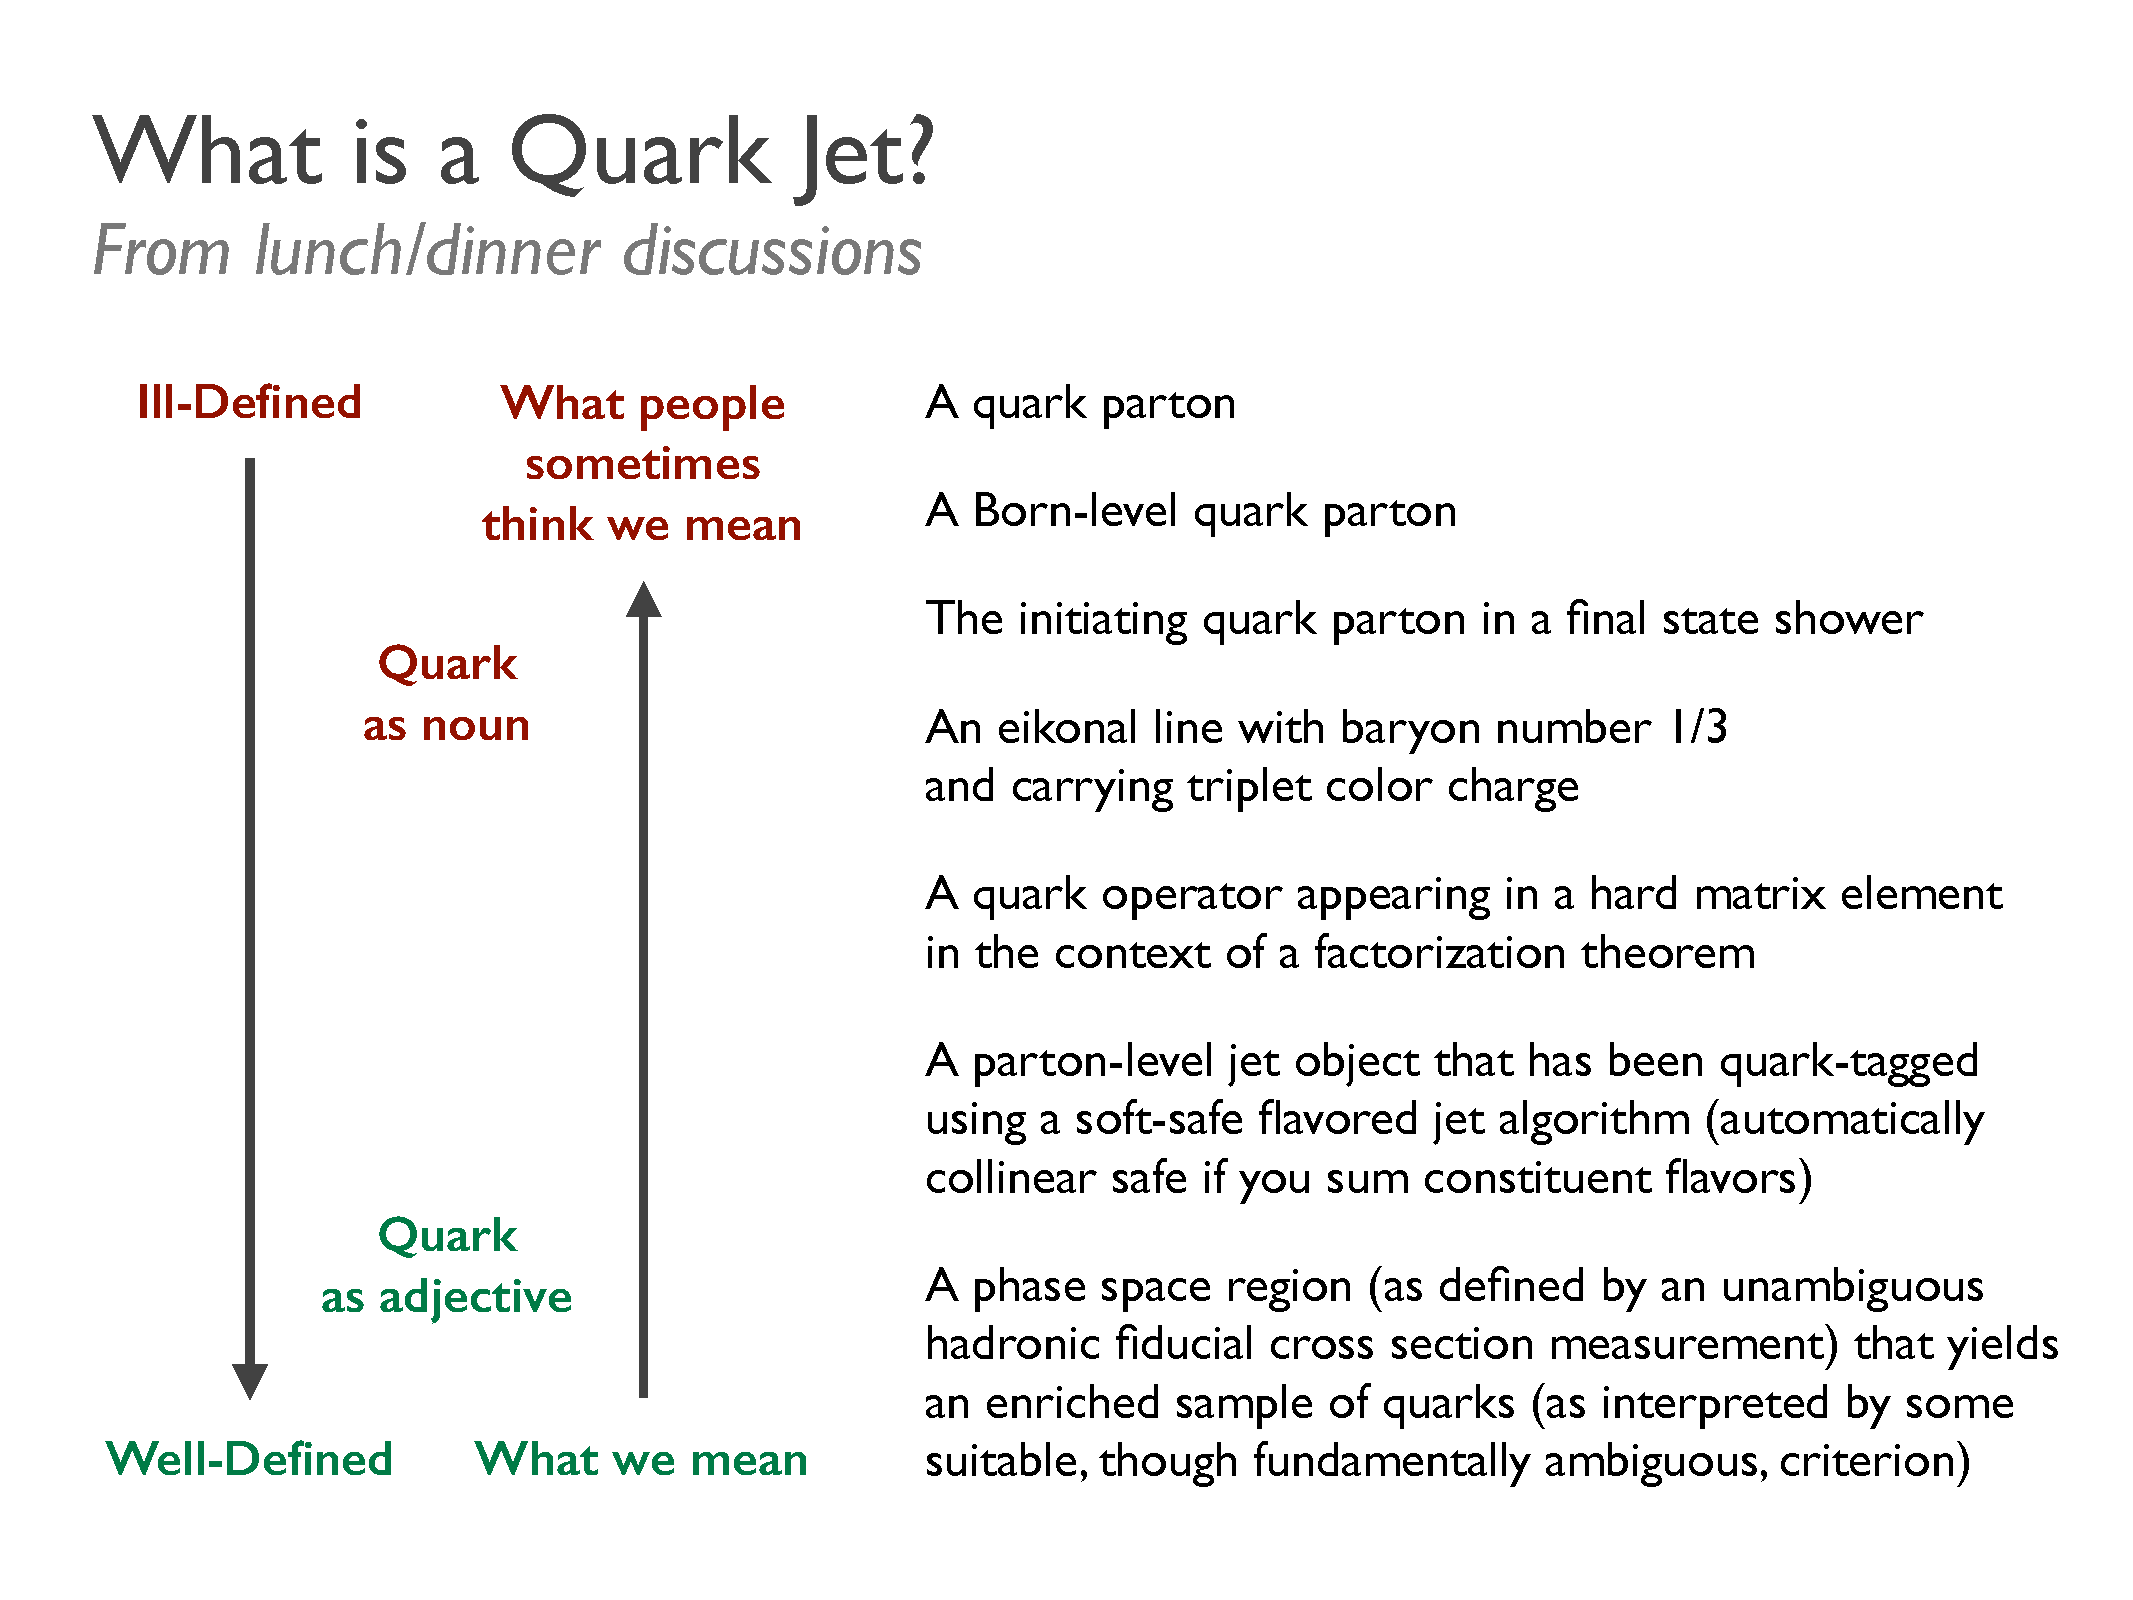
\includegraphics[width=0.7 \columnwidth]{quarkgluon_fig_summary_slide.pdf}
}
\caption{Original slide from the June 10, 2015 summary report of the quark/gluon Les Houches subgroup.}
\label{quarkgluon_fig:summary_slide}
\end{figure}

As part of the 2015 Les Houches workshop, an attempt was made to
define exactly what is meant by a ``quark jet'' or ``gluon jet'' (see Fig.~\ref{quarkgluon_fig:summary_slide}).
Here are some suggested options for defining a quark jet, in
(approximate) order from most ill-defined to most well-defined.
Related statement can be made for gluon jets.

\noindent \textbf{A quark jet is...}
\begin{itemize}
\item \textbf{A quark parton.}  This definition (incorrectly) assumes that there is a one-to-one map between a jet and its initiating parton.  Because it neglects the important role of additional radiation in determining the structure of a jet, we immediately dismiss this definition.
\item \textbf{A Born-level quark parton.}  This definition at least acknowledges the importance of radiative corrections to jet production, but it leaves open the question of how exactly to define the underlying Born-level process from an observed final state.  (For one answer valid at the parton level, see flavored jet algorithms below.)
\item \textbf{An initiating quark parton in a final state parton
    shower.}  We suspect that this is the definition most LHC
  experimentalists have in mind.  This definition assumes that the parton shower history is meaningful, though,
  which may not be the case beyond the strongly-ordered or
  leading-logarithmic approximations.  Because the parton shower is
  semi-classical, this definition neglects the impact of genuinely
  quantum radiative corrections as well as nonperturbative
  hadronization.
\item \textbf{A maximum-$p_T$ quark parton within a jet in a final state parton shower.}  This ``max-$p_T$'' prescription is a variant on the initiating parton prescription above (see further discussion in \cite{Buckley:2015gua}).  It differs from the initiating parton by a calculable amount in a leading logarithmic shower \cite{Dasgupta:2014yra} and is based on the same (naive) assumption that the parton shower history is meaningful. 
\item \textbf{An eikonal line with baryon number 1/3 and carrying triplet color charge.}  This is another semi-classical definition that attempts to use a well-defined limit of QCD to define quarks in terms of light-like Wilson lines.  Philosophically, this is similar to the parton shower picture, with a similar concern about how to extrapolate this definition away from the strict eikonal limit.
\item \textbf{A parton-level jet object that has been quark-tagged using an IRC safe flavored jet algorithm.}  This is the strategy adopted in \cite{Banfi:2006hf}.  While this definition neglects the impact of hadronization, it does allow for the calculation of quark jet cross sections at all perturbative orders, including quantum corrections.
\end{itemize}
The unifying theme in the above definitions is that they try to identify a quark as an object unto itself, without reference to the specific final state of interest.  However, it is well-known that a ``quark'' in one process may not look like a ``quark'' in other process, due to color correlations with the rest of the event, especially the initial state in $pp$ collisions.  The next definition attempts to deal with the process dependence in defining quarks. 
\begin{itemize}
\item \textbf{A quark operator appearing in a hard matrix element in the context of a factorization theorem.}  This is similar to the attitude taken in \cite{Gallicchio:2011xc}.  In the context of a well-defined cross section measurement, one can (sometimes) go to a limit of phase space where the hard production of short-distance quarks and gluons factorizes from the subsequent long-distance fragmentation.  This yields a nice (gauge-covariant) operator definition of a quark jet.  That said, even if a factorization theorem does exist for the measurement of interest, this definition is potentially ambiguous beyond leading power.
\end{itemize}
The definition we adopt for this study is inspired by the idea that one should think about quark/gluon tagging in the context of a specific measurement, but it tries to avoid relying on the presence of a factorization theorem.
\begin{itemize}
\item \textbf{A phase space region (as defined by an unambiguous
    hadronic fiducial cross section measurement) that yields an
    enriched sample of quarks (as interpreted by some suitable, though
    fundamentally ambiguous, criterion).}  Here, the goal is to
  \emph{tag} a phase space region as being quark-like, rather than try
  to determine a truth definition of a quark.  This definition has the
  advantage of being explicitly tied to hadronic final states and to
  the discriminant variables of interest. \emph{The main
  challenge with this definition is how to determine the criterion
  that corresponds to successful quark enrichment.}  For that, we will
  have to rely to some degree on the other less well-defined notions
  of what a quark jet is.
\end{itemize}

To better understand this last definition, consider a quark/gluon discriminant $\lambda$.  Since $\lambda$ can be measured on any jet, one can unambiguously determine the cross section $\text{d} \sigma / \text{d} \lambda$ for any jet sample of interest.  But measuring $\lambda$ does not directly lead to the probability that the jet is a quark jet, nor to the probability distribution  $p_q(\lambda)$ for $\lambda$ within a quark jet sample.  Rather, the process of measuring $\lambda$ must be followed by a separate process of interpreting how the value of $\lambda$ should be used as part of an analysis.

For example, the user could choose that small $\lambda$ jets should be tagged as ``quark-like'' while large $\lambda$ jets should be tagged as ``gluon-like''. Alternatively, the user might combine $\lambda$ with other discriminant variables as part of a more sophisticated classification scheme.  The key point is that one first measures hadron-level discriminant variables on a final state of interest, and only later does one interpret exactly what those discriminants accomplish (which could be different depending on this physics goals of a specific analysis).  Typically, one might use a Born-level or eikonal analysis to define which regions of phase space should be associated with ``quarks'' or ``gluons'', but even if these phase space regions are based on naive or ambiguous logic, $\lambda$ itself is a well-defined discriminant variable.

In Sec.~\ref{quarkgluon_sec:ee}, we will consider the generalized
angularities $\lambda_{\beta}^\kappa$ as our discriminant variables
and we will assess the degree to which the measured values of
$\lambda_{\beta}^\kappa$ agree with a quark/gluon interpretation based
on Born-level production modes.  This is clearly an idealization,
though one that makes some sense in the context of $e^+e^-$
collisions, since the truth-level ``quark'' and ``gluon'' labels are
defined by the Lorentz structure of the production vertex.  In
Sec.~\ref{quarkgluon_sec:conclude}, we will recommend that the LHC
experiments perform measurements of $\lambda_\beta^\kappa$ in
well-defined hadron-level final states, without necessarily attempting
to determine separate $p_q(\lambda_\beta^\kappa)$ and
$p_g(\lambda_\beta^\kappa)$ distributions.  Eventually, one would want
to use these hadron-level measurements to infer something about
parton-level quark/gluon radiation patterns.  Even without that
interpretation step, though, direct measurements of $\text{d} \sigma /
\text{d} \lambda_\beta^\kappa$ would provide valuable information for
parton shower tuning.  This in turn would help $\lambda_\beta^\kappa$ become a more robust and powerful discriminant in searches for new physics beyond the standard model. 

\subsection{Generalized Angularities}
\label{quarkgluon_sec:genang}

\begin{figure}
\centering
\subfloat{
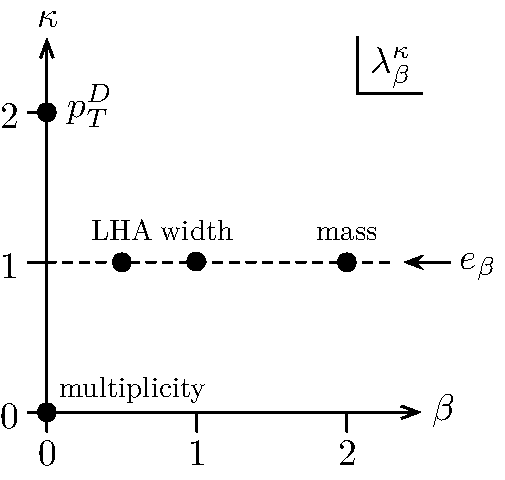
\includegraphics[scale = 0.7]{quarkgluon_fig_lambda_space.pdf}
}
\caption{Two-parameter family of generalized angularities, adapted from \cite{Larkoski:2014pca}.  The dots correspond to the five benchmark angularities used in this study.  The horizontal line at $\kappa = 1$ corresponds to the IRC safe angularities, $e_\beta = \lambda^{1}_{\beta}$.}
\label{quarkgluon_fig:lambda_space}
\end{figure}

A wide variety of quark/gluon discriminants have been proposed (see \cite{Gallicchio:2012ez} for an extensive catalog), but here we limit ourselves to a two-parameter family of generalized angularities \cite{Larkoski:2014pca}, shown in Fig.~\ref{quarkgluon_fig:lambda_space}.  These are defined as (repeating Eq.~\eqref{quarkgluon_eq:genang_intro} for convenience)
\begin{equation}
\label{quarkgluon_eq:genang}
\lambda^{\kappa}_{\beta} = \sum_{i \in \text{jet}} z_i^\kappa \theta_i^\beta,
\end{equation}
where $i$ runs over the jet constituents, $z_i \in [0,1]$ is a momentum fraction, and $\theta_i \in [0,1]$ is a (normalized) angle to the jet axis.  The parameters $\kappa \ge 0$ and $\beta \ge 0$ determine the momentum and angle weighting, respectively.  For $\kappa = 1$, the generalized angularities are IRC safe and hence calculable in perturbation theory \cite{Larkoski:2014uqa} (see also \cite{Ellis:2010rwa,Larkoski:2013paa,Larkoski:2014tva,Procura:2014cba,Hornig:2016ahz}).  For general $\kappa \not= 1$, there are quasi-perturbative techniques based on generalized fragmentation functions \cite{Larkoski:2014pca} (see also \cite{Krohn:2012fg,Waalewijn:2012sv,Chang:2013rca,Chang:2013iba}).  In our parton shower studies, we determine $\lambda^{\kappa}_{\beta}$ using all constituents of a jet, though one could also consider using charged-particle-only angularities to improve robustness to pileup (at the expense of losing some particle-level information).

For our $e^+ e^-$ study, we cluster jets with \textsc{FastJet 3.1.3} \cite{Cacciari:2011ma} using the $ee$-variant of the
anti-$k_t$ algorithm \cite{Cacciari:2008gp}, with $|\vec{p}|$-ordered
winner-take-all recombination
\cite{Larkoski:2014uqa,Bertolini:2013iqa,Salam:WTAUnpublished} to
determine the jet axis $\hat{n}$.  Unlike standard $E$-scheme
recombination \cite{Blazey:2000qt}, the winner-take-all scheme yields
a jet axis $\hat{n}$ that does not necessarily align with the jet
three-momentum $\vec{p}$; this turns out to be a desirable feature
for avoiding soft recoil effects
\cite{Larkoski:2013eya,Larkoski:2014uqa,Catani:1992jc,Dokshitzer:1998kz,Banfi:2004yd}.  We define
\begin{equation}
z_i \equiv \frac{E_i}{E_{\rm jet}}, \qquad \theta_i \equiv \frac{\Omega_{i \hat{n}}}{R},
\end{equation}
where $E_i$ is the particle energy, $\Omega_{i \hat{n}}$ is the opening angle to the jet axis, and $R$ is the jet radius (taken to be $R = 0.6$ by default).  To translate our $ee$ study to an eventual $pp$ study (left to future work), one would use the standard $pp$ version of anti-$k_t$ with $p_T$-ordered winner-take-all recombination, defining
\begin{equation}
z_i \equiv \frac{p_{Ti}}{\sum_{j \in \text{jet}} p_{Tj}}, \qquad \theta_i \equiv \frac{R_{i \hat{n}}}{R},
\end{equation}
where $p_{Ti}$ is the particle transverse momentum and $R_{i \hat{n}}$ is the rapidity-azimuth distance to the jet axis.



By adjusting $\kappa$ and $\beta$, one can probe different aspects of the jet fragmentation.  We consider five benchmark values for $(\kappa, \beta)$ indicated by the black dots in Fig.~\ref{quarkgluon_fig:lambda_space}:
\begin{equation}
\label{quarkgluon_eq:benchmarkang}
\begin{aligned}
(0,0) &= \text{hadron multiplicity},\\
(2,0) &\Rightarrow p_T^D \text{  \cite{Pandolfi:1480598,Chatrchyan:2012sn} (specifically $\lambda^{2}_{0} = (p_T^D)^2$)},\\
(1,0.5) & = \text{Les Houches Angularity (LHA)},\\
(1,1) &= \text{width or broadening \cite{Catani:1992jc,Rakow:1981qn,Ellis:1986ig}},\\
(1,2) & \Rightarrow \text{mass or thrust \cite{Farhi:1977sg}
  (specifically $\lambda^{1}_{2} \simeq m_{\rm jet}^2 / E_{\rm
    jet}^2$)}.
\end{aligned}
\end{equation}
Except for the LHA, these angularities (or their close cousins) have already been used in quark/gluon discrimination studies.  The LHA has been included to have an IRC safe angularity that weights energies more heavily than angles, similar in spirit to the $\beta = 0.2$ value advocated in Ref.~\cite{Larkoski:2013eya}.

For the IRC safe case of $\kappa = 1$, there is an alternative version
of the angularities based on energy correlation functions \cite{Larkoski:2013eya} (see also \cite{Banfi:2004yd,Jankowiak:2011qa}),
\begin{equation}
\text{ecf}_\beta = \sum_{i < j \in \text{jet}} z_i z_j \theta_{ij}^\beta \simeq \lambda^{1}_{\beta},
\end{equation}
where equality holds in the extreme eikonal limit.\footnote{This equality also relies on using a recoil-free axis choice $\hat{n}$ to define $\theta_i$.  Amusingly, $\lim_{\beta \to 0} \text{ecf}_\beta = (1 - \lambda^{2}_{0})/2$ (i.e.~$\kappa = 2$, $\beta = 0$), such that the $\beta \to 0$ limit of the IRC safe energy correlation functions corresponds to the IRC unsafe $p_T^D$.}  For the $e^+ e^-$ case, the pairwise angle $\theta_{ij}$ is typically normalized to the jet radius as $\theta_{ij} \equiv \Omega_{ij}/R$.   To avoid a proliferation of curves, we will not show any results for $\text{ecf}_\beta$.  We will also neglect quark/gluon discriminants that take into account azimuthal asymmetries within the jet, though observables like the covariance tensor \cite{Gallicchio:2012ez} and 2-subjettiness \cite{Thaler:2010tr,Thaler:2011gf} can improve quark/gluon discrimination.

\subsection{Classifier Separation}
\label{quarkgluon_sec:classsep}

Since we will be testing many parton shower variants, we need a way to quantify quark/gluon separation power in a robust way that can easily be summarized by a single number.  For that purpose we use classifier separation  (repeating Eq.~\eqref{quarkgluon_eq:deltadef_intro} for convenience),
\begin{equation}
\label{quarkgluon_eq:deltadef}
\Delta =  \frac{1}{2} \int \text{d} \lambda \, \frac{\bigl(p_q(\lambda) - p_g(\lambda)\bigr)^2}{p_q(\lambda) + p_g(\lambda)},
\end{equation}
where $p_q$ ($p_g$) is the probability distribution for the quark jet (gluon jet) sample as a function of the classifier $\lambda$.  Here, $\Delta = 0$ corresponds to no discrimination power and $\Delta = 1$ corresponds to perfect discrimination power.

A more common way to talk about discrimination power is in terms of receiver operating characteristic (ROC) curves.  At a point ($q$,$g$) on the ROC curve, where $q,g \in [0,1]$, one can define a selection that yields $q$ efficiency for quarks and $g$ mistag rate for gluons, or equivalently, a $(1-g)$ efficiency for gluons for a $(1-q)$ mistag rate for quarks.  To turn the ROC curve into a single number, it is common to report the gluon rejection rate at, say, 50\% quark efficiency.  Since we are more interested in understanding the relative performance between parton showers rather than the absolute performance, we will not show ROC curves here, though they can be easily derived from the $p_q$ and $p_g$ distributions.  If one observable has an everywhere better ROC curve than another (i.e.~it is Pareto optimal), then it will also have a larger $\Delta$ value.  The converse is not true, however, since depending on the desired working point, a ``bad'' discriminant as measured by $\Delta$ might still be ``good'' by another metric.  In that sense, $\Delta$ contains less information than the full ROC curve.

An alternative way to quantify discrimination power is through mutual information, which counts the number of ``bits'' of information gained from measuring a discriminant variable (see \cite{Larkoski:2014pca}).  Given a sample with quark fraction $f \in [0,1]$ and gluon fraction $(1-f)$, the mutual information with the truth (a.k.a. the truth overlap) is
\begin{equation}
I(T; \Lambda) = \int \text{d} \lambda \left(f \, p_q(\lambda) \log_2 \frac{p_q(\lambda)}{p_{\rm tot}(\lambda)} + (1-f) \, p_g(\lambda) \log_2 \frac{p_g(\lambda)}{p_{\rm tot}(\lambda)}   \right),
\end{equation}
where $T = \{q,g\}$ is the set of truth labels, $\Lambda = \{\lambda\}$ is the (continuous) set of discriminant values, and 
\begin{equation}
p_{\rm tot}(\lambda) = f \, p_q(\lambda) + (1-f) \, p_g(\lambda).
\end{equation}
The choice $f = 1/2$ was used in Ref.~\cite{Larkoski:2014pca}, though other $f$ choices are plausible.  Though we will not use mutual information in this study, it is amusing to note that the second derivative of $I(T;\Lambda)$ with respect to $f$ is related to classifier separation as
\begin{equation}
\label{quarkgluon_eq:altdeltadef}
- \frac{\log 2}{4} \frac{\partial^2 I(T;\Lambda)}{\partial f^2} \Big|_{f = \frac{1}{2}} = \Delta.
\end{equation}

One advantage of $\Delta$ over $I(T;\Lambda)$ is that the integrand in Eq.~\eqref{quarkgluon_eq:deltadef} is easier to interpret, since it tracks the fractional difference between the signal and background at a given value of $\lambda$.\footnote{Another advantage of $\Delta$ over $I(T; \Lambda)$ arises when trying to assign statistical uncertainties to finite Monte Carlo samples.  Since $\Delta$ is defined as a simple integral, one can use standard error propagation to assign uncertainties to $\Delta$.  By contrast, because of the logarithms in the $I(T; \Lambda)$ integrand, one has to be careful about a potential binning bias \cite{Larkoski:2014pca}.}  Specifically, by plotting 
\begin{equation}
\label{quarkgluon_eq:deltaintegrand}
\frac{\text{d} \Delta}{\text{d} \lambda} = \frac{1}{2} \frac{\bigl(p_q(\lambda) - p_g(\lambda) \bigr)^2}{p_q(\lambda) + p_g(\lambda)},
\end{equation}
one can easily identify which regions of phase space contribute the most to quark/gluon discrimination.  One can then ask whether or not the regions exhibiting the most separation power are under sufficient theoretical control, including both the size of perturbative uncertainties and the impact of nonperturbative corrections.  

\subsection{Idealized Quark/Gluon Discrimination}
\label{quarkgluon_sec:ee}

Our parton shower studies are based on the idealized case of discriminating quark and gluon jets in $e^+ e^-$ collisions.  As we will see, this example demonstrates the importance of final state evolution for quark/gluon discrimination, separate from initial state complications arising in $pp$ collisions.  The analysis code used for this study is available as a \textsc{Rivet} routine \cite{Buckley:2010ar}, which can be downloaded from \verb|https://github.com/gsoyez/lh2015-qg| under \verb|MC_LHQG_EE.cc|.

To define the truth-level jet flavor, we use a simple definition:  a quark jet is a jet produced by a parton shower event generator in $e^+ e^- \to (\gamma/Z)^* \to u \bar{u}$ hard scattering, while a gluon jet is a jet produced in $e^+ e^- \to h^* \to gg$.  Of course, an $e^+e^- \to u \bar u$ event can become a $e^+e^- \to u \bar u g$ event after one step of shower evolution, just as $e^+e^- \to g g$ can become $e^+e^- \to g u \bar u$.  This illustrates the inescapable ambiguity in defining jet flavor.\footnote{In an $e^+e^-$ context, our definition at least respects the Lorentz structure of the production vertex, so in that sense it is a fundamental definition that does not reference (ambiguous) quark or gluon partons directly.}  To partially mitigate the effect of wide-angle emissions, we restrict our analysis to jets that satisfy
\begin{equation}
\frac{E_{\rm jet}}{Q/2} > 0.8,
\end{equation}
with up to two jets studied per event.  There is also the ambiguity of which parton shower to use, and we investigate this ambiguity by looking at results from several event generators:  \textsc{Pythia 8.205} \cite{Sjostrand:2006za,Sjostrand:2014zea}, \textsc{Herwig++ 2.7.1} \cite{Bahr:2008pv,Bellm:2013hwb}, \textsc{Sherpa 2.1.1} \cite{Gleisberg:2008ta}, \textsc{Vincia 1.201} \cite{Giele:2013ema}, \textsc{Deductor 1.0.2} \cite{Nagy:2014mqa} (with hadronization performed by \textsc{Pythia}), and \textsc{Ariadne 5.0.$\beta$} \cite{Flensburg:2011kk}.  

\begin{figure}
\centering
\subfloat[]{
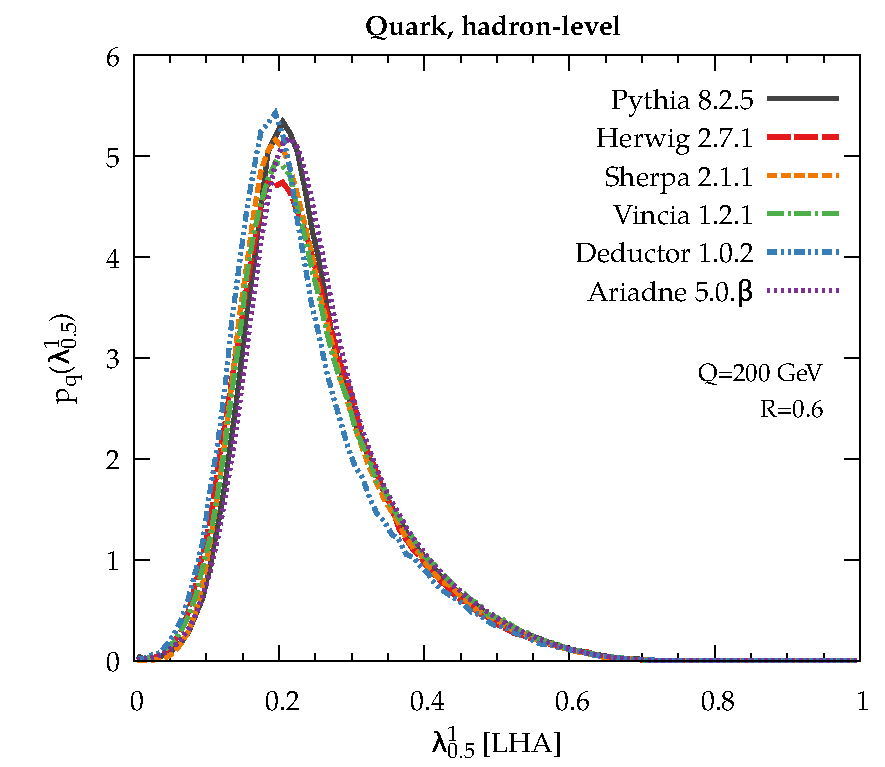
\includegraphics[width = 0.45\columnwidth]{quarkgluon_fig_GA_10_05_R6_hadron_quark.pdf}
\label{quarkgluon_fig:LHA_hadron_quark}
}
$\qquad$
\subfloat[]{
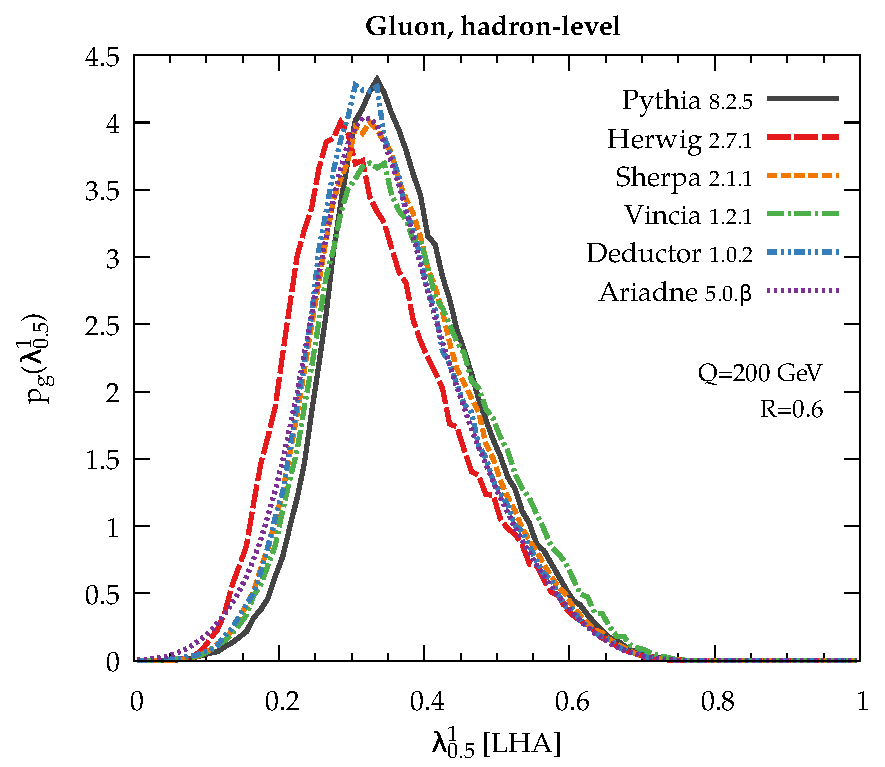
\includegraphics[width = 0.45\columnwidth]{quarkgluon_fig_GA_10_05_R6_hadron_gluon.pdf}
\label{quarkgluon_fig:LHA_hadron_gluon}
}

\subfloat[]{
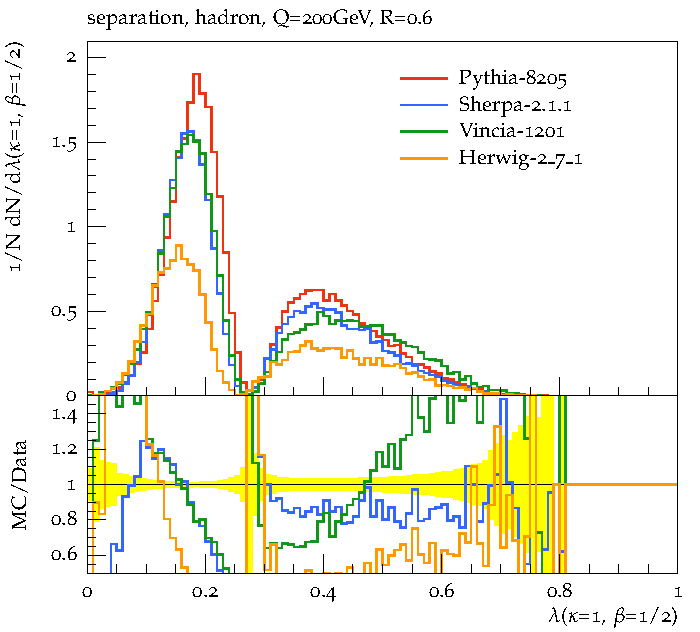
\includegraphics[width = 0.65\columnwidth]{quarkgluon_fig_GA_10_05_R6_hadron_separation.pdf}
\label{quarkgluon_fig:LHA_hadron_separation}
}
\caption{Hadron-level distributions of the LHA for (a) the $e^+ e^- \to u \bar{u}$ (``quark jet'') sample, (b) the $e^+ e^- \to gg$ (``gluon jet'') sample, and (c) the classifier separation integrand in Eq.~\eqref{quarkgluon_eq:deltaintegrand}.  Six parton shower generators---\textsc{Pythia 8.205}, \textsc{Herwig++ 2.7.1}, \textsc{Sherpa 2.1.1}, \textsc{Vincia 1.201}, \textsc{Deductor 1.0.2}, and \textsc{Ariadne 5.0.$\beta$}---are run at their baseline settings with center-of-mass energy $Q = 200~\GeV$ and jet radius $R= 0.6$.}
\label{quarkgluon_fig:LHA_hadron}
\end{figure}

In Fig.~\ref{quarkgluon_fig:LHA_hadron}, we show hadron-level distributions of the LHA (i.e.~$\lambda_{0.5}^1$) in the quark sample ($p_q$) and gluon sample ($p_g$), comparing the baseline settings of six different parton shower generators with a center-of-mass collision energy of $Q = 200~\GeV$ and jet radius $R = 0.6$. In the quark sample in Fig.~\ref{quarkgluon_fig:LHA_hadron_quark}, there is relatively little variation between the generators, which is not surprising since most of these programs have been tuned to match LEP data (though LEP never measured the LHA itself).  Turning to the gluon sample in Fig.~\ref{quarkgluon_fig:LHA_hadron_gluon}, we see somewhat larger variations between the generators; this is expected since there is no data to directly constrain $e^+ e^- \to gg$.  In Fig.~\ref{quarkgluon_fig:LHA_hadron_separation}, we plot the integrand of classifier separation, $\text{d} \Delta / \text{d} \lambda$ from Eq.~\eqref{quarkgluon_eq:deltaintegrand}. This shows where in the LHA phase space the actual discrimination power lies, with large values of the integrand
corresponding to places where the quark and gluon distributions are
most dissimilar.  Now we see considerable differences between the
generators, reproducing the well-known fact that \textsc{Pythia} is
more optimistic about quark/gluon separation compared to
\textsc{Herwig} \cite{Aad:2014gea}.  The predicted discrimination power from the other four generators are intermediate between these
extremes.

\begin{figure}
\centering
\subfloat[]{
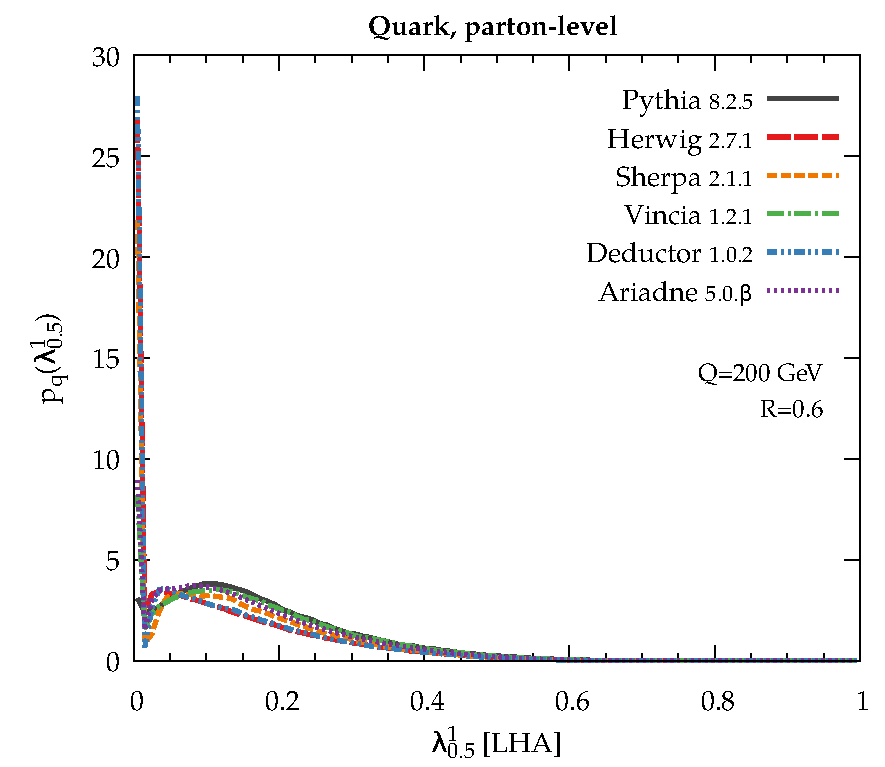
\includegraphics[width = 0.45\columnwidth]{quarkgluon_fig_GA_10_05_R6_parton_quark.pdf}
\label{quarkgluon_fig:LHA_parton_quark}
}
$\qquad$
\subfloat[]{
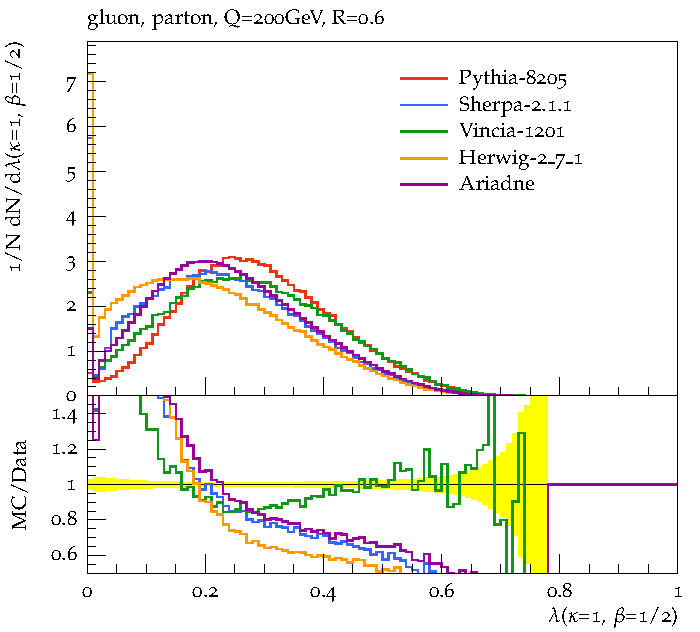
\includegraphics[width = 0.45\columnwidth]{quarkgluon_fig_GA_10_05_R6_parton_gluon.pdf}
\label{quarkgluon_fig:LHA_parton_gluon}
}

\subfloat[]{
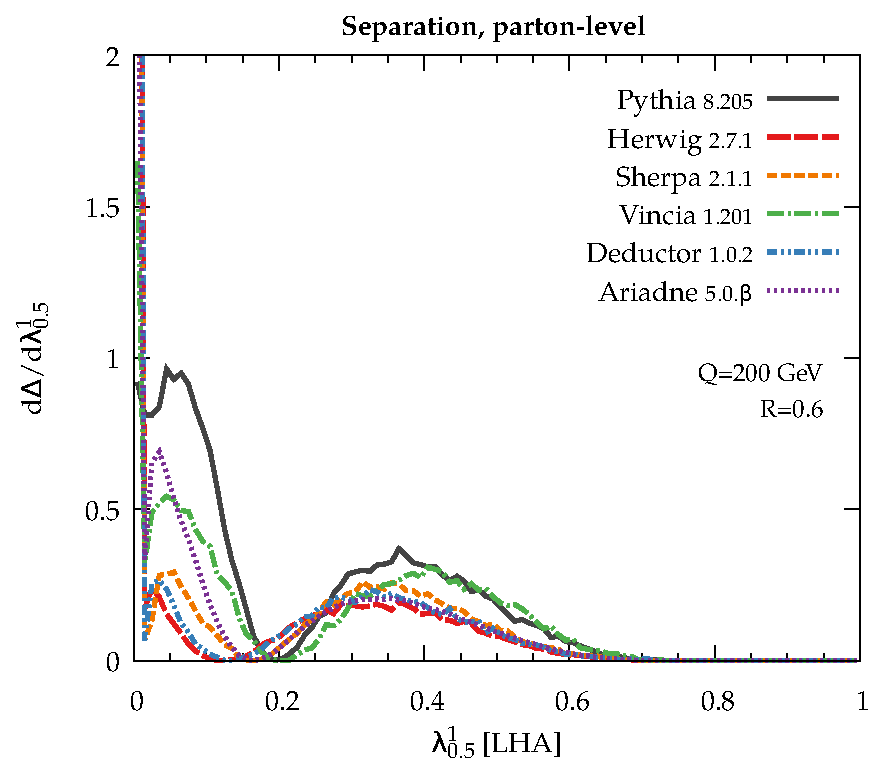
\includegraphics[width = 0.65\columnwidth]{quarkgluon_fig_GA_10_05_R6_parton_separation.pdf}
\label{quarkgluon_fig:LHA_parton_separation}
}
\caption{Same as Fig.~\ref{quarkgluon_fig:LHA_hadron}, but at the parton level.  Note that \textsc{Herwig}, \textsc{Sherpa}, and \textsc{Deductor} all have cross section spikes at $\lambda_{0.5}^1 = 0$ that extend above the plotted range.}
\label{quarkgluon_fig:LHA_parton}
\end{figure}

One might expect that the differences between generators are due
simply to their having different hadronization models.  It seems,
however, that the differences already appear at the parton level prior
to hadronization. We should say at the outset that it is nearly impossible to do a true apples-to-apples comparison of parton-level results, since these generators are interfaced to different hadronization models, and only the hadron-level comparison is physically meaningful.  In particular, the crossover between the perturbative and nonperturbative regions is ambiguous and each of these showers has a different effective shower cutoff scale, resulting in different amounts of radiation being generated in the showering versus hadronization steps.

With that caveat in mind, we show parton-level results in Fig.~\ref{quarkgluon_fig:LHA_parton}.  One immediately notices that three of the
generators---\textsc{Herwig}, \textsc{Sherpa}, and
\textsc{Deductor}---yield a large population of events where the
perturbative shower generates no emissions.  This gives
$\lambda_{0.5}^1 = 0$ such that non-zero values of the LHA are
generated only by the hadronization model.  By contrast,
\textsc{Pythia} and \textsc{Vincia} give overall larger values of the
LHA from the perturbative shower alone.  As mentioned above, some of this difference can be explained simply by the different shower cutoff scales used in each generator, but it probably also reflects a difference in how semi-perturbative gluon splittings are treated.  Since Fig.~\ref{quarkgluon_fig:LHA_hadron_quark} shows that all generators give similar distributions for quark jets after hadronization, we
conclude that understanding quark/gluon discrimination is a challenge
at the interface between perturbative showering and nonperturbative
hadronization.

\begin{figure}
\centering
\subfloat{
\label{quarkgluon_fig:summary_hadron_all}
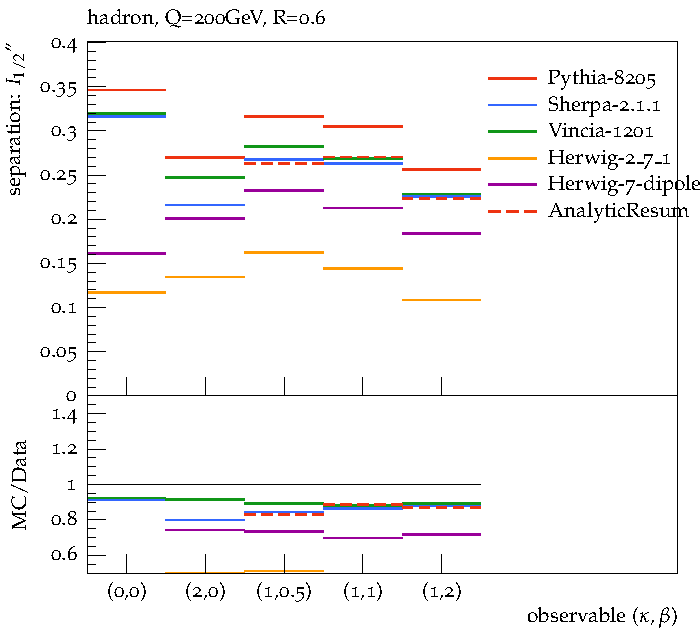
\includegraphics[width = 0.45\columnwidth]{quarkgluon_fig_I2_R6_hadron__all.pdf}
}
$\qquad$
\subfloat{
\label{quarkgluon_fig:summary_parton_all}
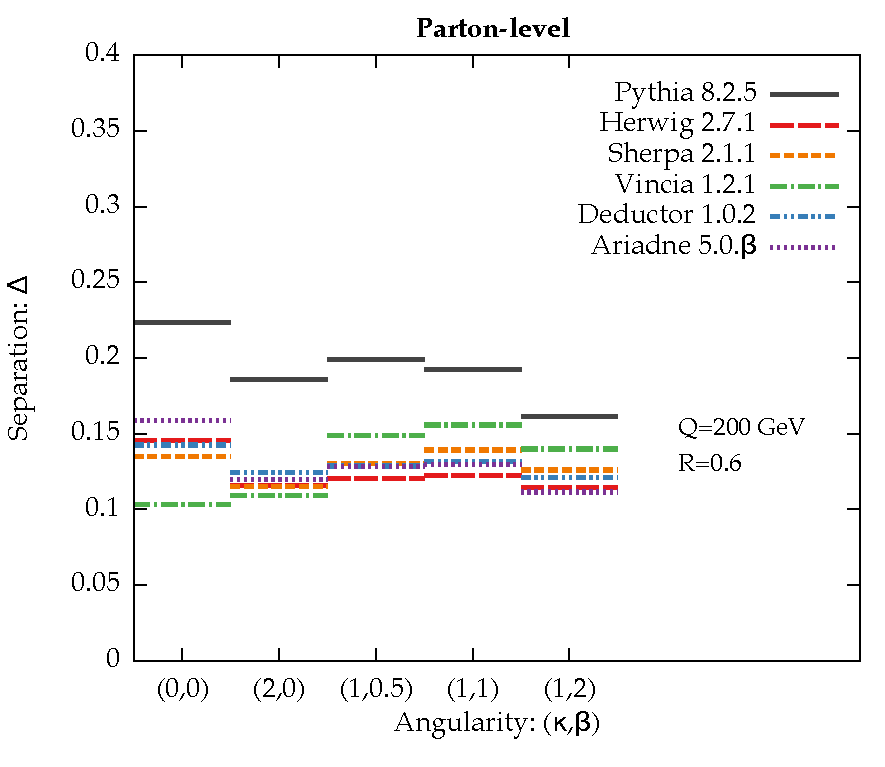
\includegraphics[width = 0.45\columnwidth]{quarkgluon_fig_I2_R6_parton__all.pdf}
}
\caption{Classifier separation $\Delta$ for the five benchmark angularities in Eq.~\eqref{quarkgluon_eq:benchmarkang}, determined from the various generators at (a) hadron level and (b) parton level.  The first two columns correspond to IRC unsafe distributions (multiplicity and $p_T^D$), while the last three columns are the IRC safe angularities.  The LHA (i.e.~$\kappa = 1$, $\beta = 1/2$) is shown in the middle column.}
\label{quarkgluon_fig:summary_all}
\end{figure}

To summarize the overall discrimination power, we integrate
Eq.~\eqref{quarkgluon_eq:deltaintegrand} to obtain the value of
classifier separation $\Delta$ for the LHA.  This is shown in
Fig.~\ref{quarkgluon_fig:summary_all}, which also includes the four
other benchmark angularities from
Eq.~\eqref{quarkgluon_eq:benchmarkang}.  There is a rather large
spread in predicted discrimination power between the generators,
especially at hadron level in
Fig.~\ref{quarkgluon_fig:summary_hadron_all}.  While such differences
might be expected for IRC unsafe angularities (multiplicity and
$p_T^D$) which depend on nonperturbative modeling, these differences
persist even for the IRC safe angularities at parton level (see
Fig.~\ref{quarkgluon_fig:summary_parton_all}).\footnote{It is interesting that four of the generators---\textsc{Herwig}, \textsc{Sherpa}, \textsc{Deductor}, and \textsc{Ariadne}---have a comparatively narrow spread in predicted discrimination power at parton level, though this spread increases dramatically at hadron level.}  This suggests a more
fundamental difference between the generators that is already present
in the perturbative shower

For the IRC safe angularities with $\kappa = 1$, there is a generic trend seen by all of the hadron-level generators that discrimination power decreases as $\beta$ increases.  This trend agrees with the study performed in Ref.~\cite{Larkoski:2013eya}, but disagrees with the ATLAS study in Ref.~\cite{Aad:2014gea}, which found flat (or even increasing) discrimination power with increasing $\beta$.  Understanding this $\beta$ trend will therefore be crucial for understanding quark/gluon radiation patterns.

\subsection{Parameter Dependence}
\label{quarkgluon_sec:ee_scales}

\begin{figure}
\centering
\subfloat[]{
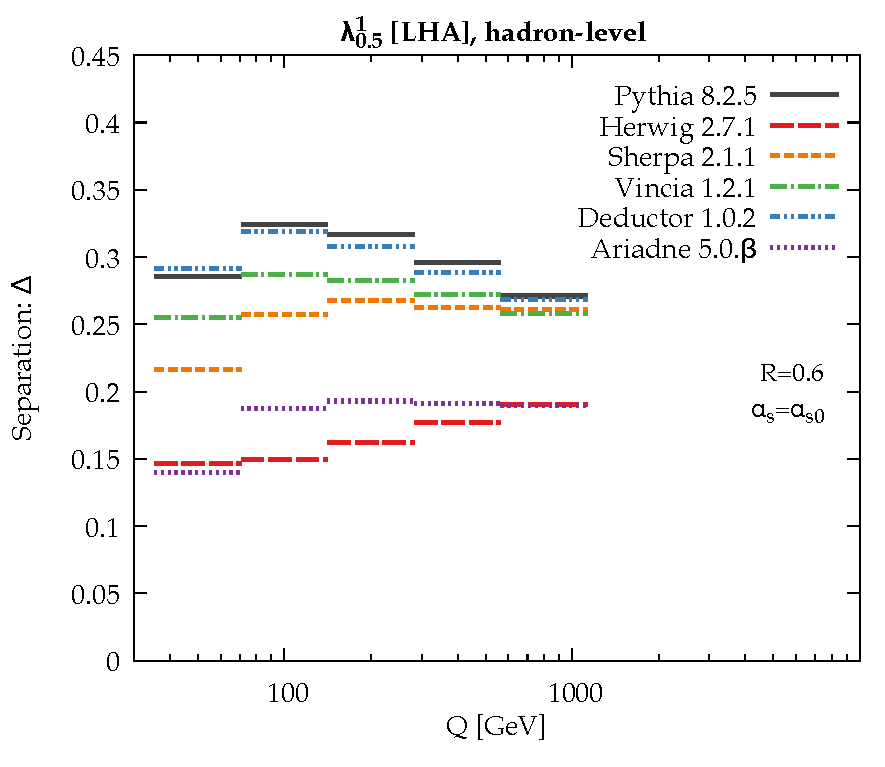
\includegraphics[width = 0.45\columnwidth]{quarkgluon_fig_I2_GA_10_05_hadron_Qdep.pdf}
\label{quarkgluon_fig:sweep_Q_hadron}
}
$\qquad$
\subfloat[]{
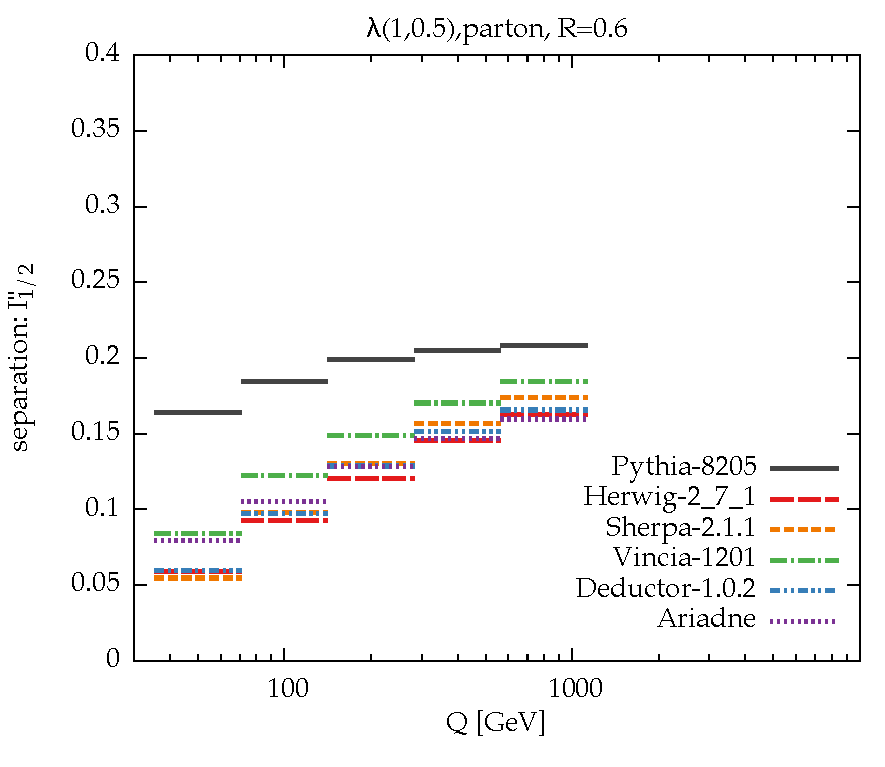
\includegraphics[width = 0.45\columnwidth]{quarkgluon_fig_I2_GA_10_05_parton_Qdep.pdf}
\label{quarkgluon_fig:sweep_Q_parton}
}

\subfloat[]{
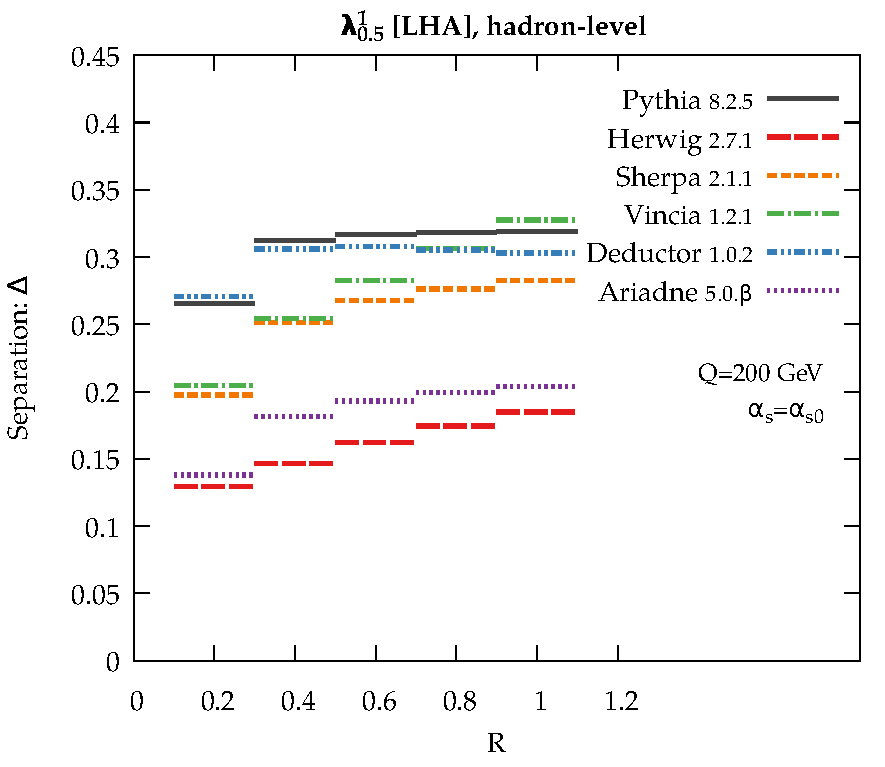
\includegraphics[width = 0.45\columnwidth]{quarkgluon_fig_I2_GA_10_05_hadron_Rdep.pdf}
\label{quarkgluon_fig:sweep_R_hadron}
}
$\qquad$
\subfloat[]{
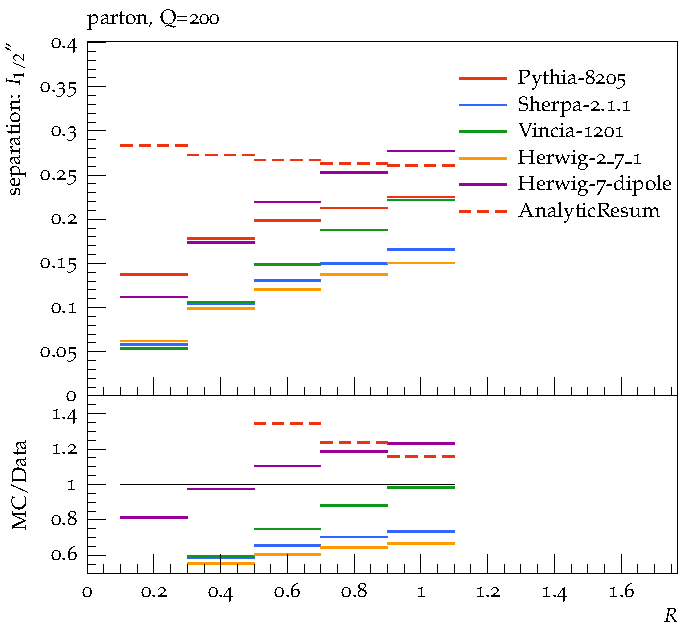
\includegraphics[width = 0.45\columnwidth]{quarkgluon_fig_I2_GA_10_05_parton_Rdep.pdf}
\label{quarkgluon_fig:sweep_R_parton}
}

\subfloat[]{
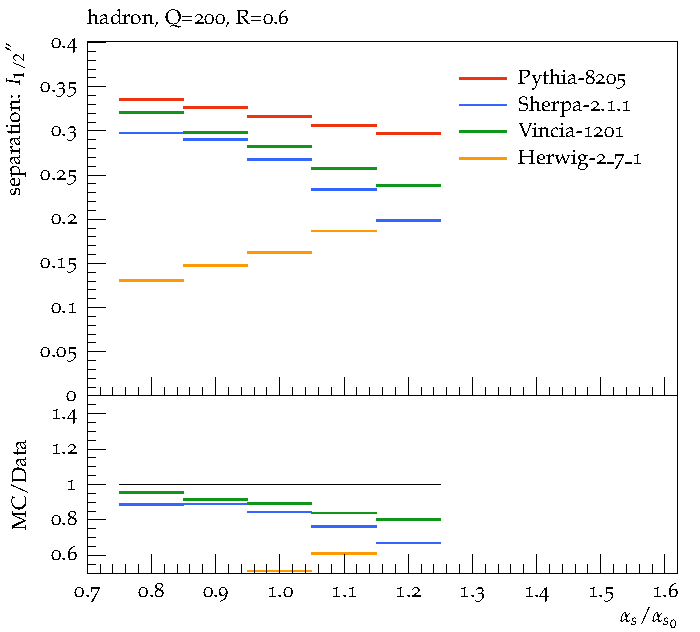
\includegraphics[width = 0.45\columnwidth]{quarkgluon_fig_I2_GA_10_05_hadron_alphadep.pdf}
\label{quarkgluon_fig:sweep_as_hadron}
}
$\qquad$
\subfloat[]{
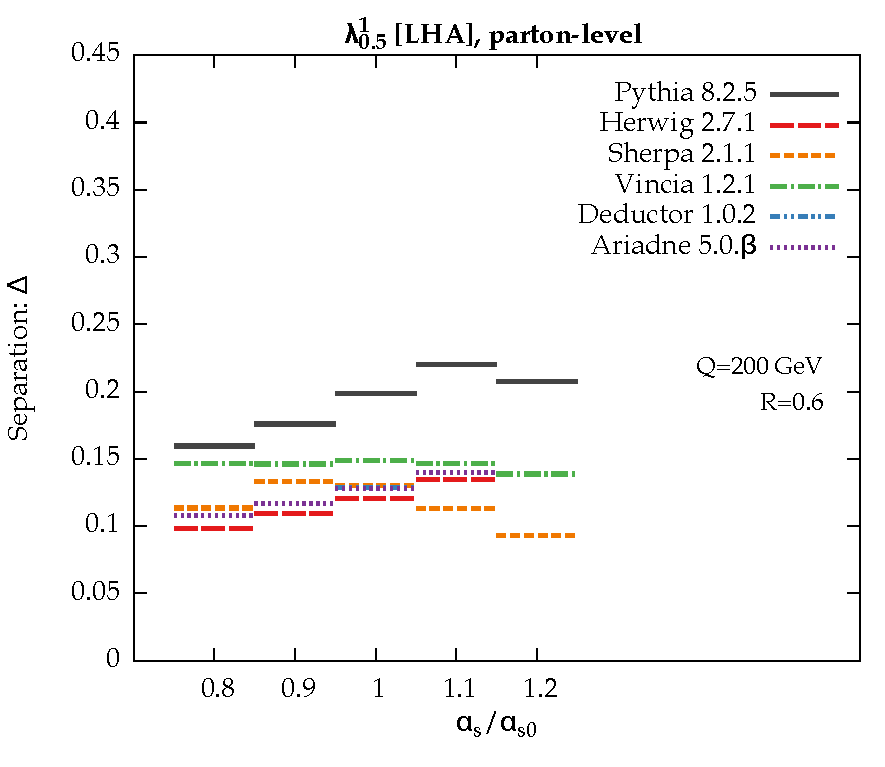
\includegraphics[width = 0.45\columnwidth]{quarkgluon_fig_I2_GA_10_05_parton_alphadep.pdf}
\label{quarkgluon_fig:sweep_as_parton}
}
\caption{Classifier separation $\Delta$ for the LHA, sweeping the collision energy $Q$ (top row), jet radius $R$ (middle row), and coupling constant $\alpha_s/\alpha_{s0}$ (bottom row).  Results are shown at hadron level (left column) and parton level (right column).}
\label{quarkgluon_fig:ee_sweep}
\end{figure}

Given the large absolute differences in discrimination power seen above, we next want to check if the parton shower generators exhibit similar or dissimilar trends as parameters are varied.  We perform three parameter sweeps, using the boldface values below as defaults:
\begin{equation}
\begin{aligned}
\text{Collision Energy}: Q &= \{ 50, 100, \mathbf{200}, 400, 800\}~\GeV, \\
\text{Jet Radius}: R &= \{ 0.2, 0.4, \mathbf{0.6}, 0.8, 1.0\}, \\
\text{Strong Coupling}: \alpha_s / \alpha_{s0} &= \{0.8,0.9,\mathbf{1.0},1.1,1.2\}, \\
\end{aligned}
\end{equation}
where $\alpha_{s0}$ is the default value of the strong coupling, which is different between the generators (and sometimes different between different aspects of the same generator).

The resulting values of $\Delta$ for the LHA are shown in Fig.~\ref{quarkgluon_fig:ee_sweep}, at both the hadron level and parton level.   There are number of surprising features in these plots.  Perhaps the most obvious (and seen already in Fig.~\ref{quarkgluon_fig:summary_all}) is that even for the IRC safe angularities, the effect of hadronization is rather large, both on the absolute scale of discrimination and the trends.  The main exception to this is \textsc{Herwig}, which does not exhibit as much of an effect from hadronization, though an effect is still present.

The next surprising feature is that the parton-level trends for sweeping $\alpha_s$ do not necessarily correspond to those for sweeping $Q$ and $R$.  According to the perturbative next-to-leading-logarithmic (NLL) logic in Ref.~\cite{Larkoski:2013eya}, quark/gluon discrimination should depend on $\alpha_s$ evaluated at the scale $Q R / 2$, with larger values of $\alpha_s(Q R / 2)$ leading to improved discrimination power.  Indeed, \textsc{Pythia}, \textsc{Herwig}, and \textsc{Ariadne} do show improved performance with larger $\alpha_s$.  However, larger values of $Q$ and $R$ correspond to smaller values of $\alpha_s$, so the NLL logic would predict that increasing $Q$ or $R$ should lead to worse discrimination power.  Instead, all of the generators show the opposite trend.

One reason to expect quark/gluon discrimination to improve as higher energies is that that phase space available for shower evolution increases as $Q$ increases.  The scale $\mu$ of the shower splitting is $\mu_0^2 < \mu^2 < Q^2$, where $\mu_0 = \mathcal{O}(\GeV)$ is the shower cutoff scale.  With more range for shower evolution at higher $Q$, there is a greater possibility to see that a quark jet is different from a gluon jet.  Similarly, larger values of $R$ allow for more emissions within a jet, and from scaling symmetry, one expects that parton-level discrimination power should depend on the combination $Q R$.\footnote{At small values of $R$, one has to worry about the flavor purity of a jet sample, since scale evolution can change the leading parton flavor \cite{Dasgupta:2014yra,Dasgupta:2016bnd}.}  By contrast, the NLL logic says that quark/gluon discrimination should be dominated by the leading emission(s) in a jet, and since $\alpha_s$ is smaller at higher values of $Q R$, those leading emissions are more similar between quarks and gluons.  Given these two different but equally plausible logics, both of which probably play some role in the complete story, this motivates experimental tests of quark/gluon separation as a function of $Q$ and $R$.

For many of the generators, going from parton-level to hadron-level reverses or flattens the $Q$ and $\alpha_s$ trends, though the $R$ trends are more stable.  The study in Ref.~\cite{Larkoski:2013eya} did not include nonperturbative hadronization corrections, so we do not yet have a theoretical expectation for the impact of hadronization.  In future work, we plan to follow Ref.~\cite{Larkoski:2013paa} and include nonperturbative hadronization corrections via shape functions~\cite{Manohar:1994kq, Dokshitzer:1995zt, Korchemsky:1999kt, Korchemsky:2000kp, Salam:2001bd, Lee:2006nr, Mateu:2012nk} as well as test the impact of imposing a hard IR cutoff scale.  With confusions already at parton level, though, further perturbative calculations beyond NLL accuracy are also needed.  For example, at NLL accuracy, one does account for the fact that a jet can contain multiple perturbative emissions, but those emissions are treated as if they themselves do not radiate.  By contrast, parton showers allow every emission to reradiate, which might be driving the $Q$ and $R$ discrimination trends.

\subsection{Impact of Generator Settings}
\label{quarkgluon_sec:ee_settings}

Formally, parton shower generators are only accurate to modified leading-logarithmic (MLL) accuracy, though they include physically important effects like energy/momentum conservation and matrix element corrections that go beyond MLL.  We can assess the impact of these higher-order effects by changing the baseline parameter settings in each parton shower generator.  

Because each generator is different, we cannot always make the same changes for each generator.  Similarly, the spread in discrimination power shown below should \emph{not} be seen as representing the intrinsic uncertainties in the shower, since many of these changes we explore are not physically motivated.  The goal of these plots is to demonstrate possible areas where small parameter changes could have a large impact on quark/gluon discrimination.  Ultimately, collider data and higher-order calculations will be essential for understanding the origin of quark/gluon differences.  In all cases, we show both hadron-level and parton-level results, even if a setting is only expected to have an impact at the hadron level.  

\begin{figure}
\centering
\subfloat[]{
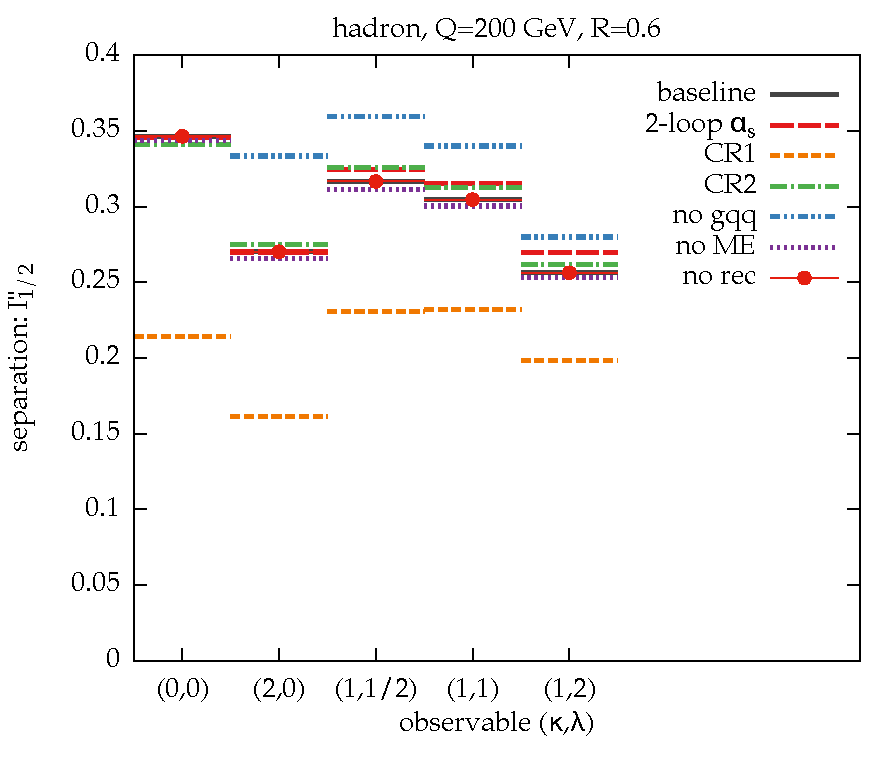
\includegraphics[width = 0.45\columnwidth]{quarkgluon_fig_I2_R6_hadron_pythia.pdf}
\label{quarkgluon_fig:summary_hadron_pythia}
}
$\qquad$
\subfloat[]{
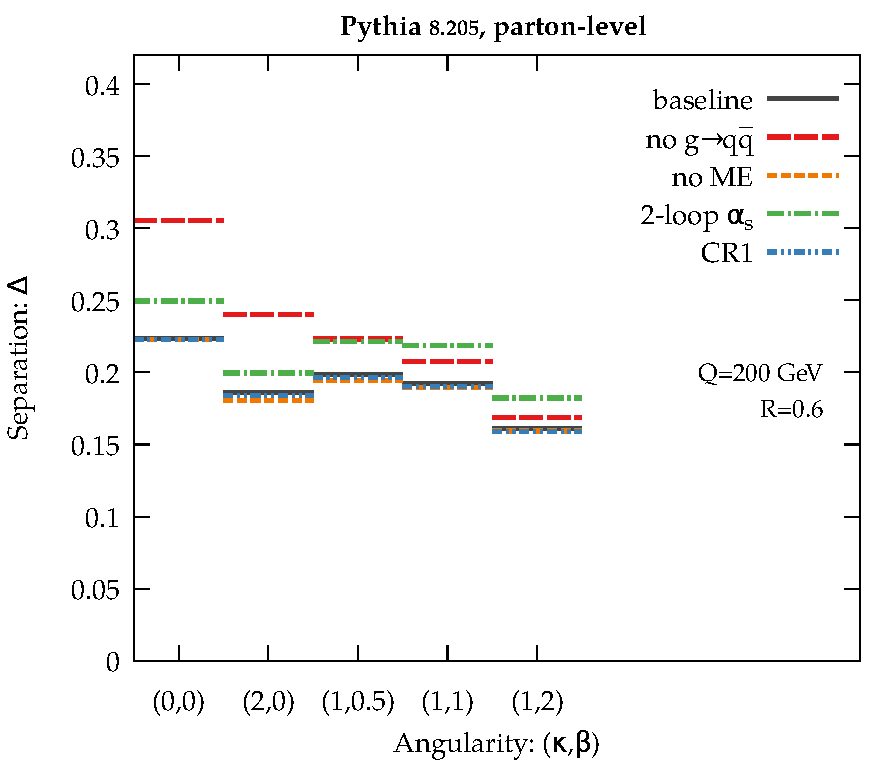
\includegraphics[width = 0.45\columnwidth]{quarkgluon_fig_I2_R6_parton_pythia.pdf}
\label{quarkgluon_fig:summary_parton_pythia}
}
\caption{Settings variations for \textsc{Pythia 8.205}.  Shown are (a) hadron-level and (b) parton-level results for the classifier separation $\Delta$ derived from the five benchmark angularities.}
\label{quarkgluon_fig:settings_variation_pythia}
\end{figure}

Our $\textsc{Pythia}$ baseline is based on the Monash 2013 tune, with parameters described in Ref.~\cite{Skands:2014pea}.  In Fig.~\ref{quarkgluon_fig:settings_variation_pythia}, we consider the following \textsc{Pythia} variations:
\begin{itemize}
\item \textsc{Pythia: no $g \to q\bar{q}$}.  While the dominant gluon splitting in the parton shower is $g \to gg$, \textsc{Pythia}---and every other shower in this study---also generates the subleading $g \to q \bar{q}$ splittings by default.  This variation turns off $g \to q \bar{q}$, which makes gluon jets look more gluon-like, thereby increasing the separation power.
\item \textsc{Pythia: no ME}.  The first emission in \textsc{Pythia} is improved by applying a matrix element correction \cite{Miu:1998ju}, but this variation turns those corrections off, showing the impact of non-singular terms.  No matrix element correction is available for $h^* \to g g$, though, so the true impact of these corrections might be larger than the relatively small effect seen for this variation.
\item \textsc{Pythia: 2-loop $\alpha_s$}.  The default \textsc{Pythia} setting is to use 1-loop running for $\alpha_s$.  This variation turns on 2-loop running for $\alpha_s$, which has a small (beneficial) effect at parton level which is washed out at hadron level.
\item \textsc{Pythia: CR1}.  Often, one thinks of color reconnection as being primarily important for hadron colliders, but even at a lepton collider, color reconnection will change the Lund strings used for hadronization.  Compared to the baseline, this variation uses an alternative ``\text{SU}(3)''-based color reconnection model~\cite{Christiansen:2015yqa} (i.e.~\texttt{ColourReconnection:mode = 1}).  No attempts were made to retune any of the other hadronization parameters (as would normally be mandated in a tuning context), so this change simply illustrates the effect of switching on this reconnection model with default parameters, leaving all other parameters unchanged.  At parton level, this variation has no effect as expected.  At hadron level, this variation considerably decreases quark/gluon separation compared to the baseline.
\end{itemize}
The most surprising \textsc{Pythia} effect is the large potential impact of the color reconnection model, which is also important for the \textsc{Herwig} generator described next.

\begin{figure}
\centering
\subfloat[]{
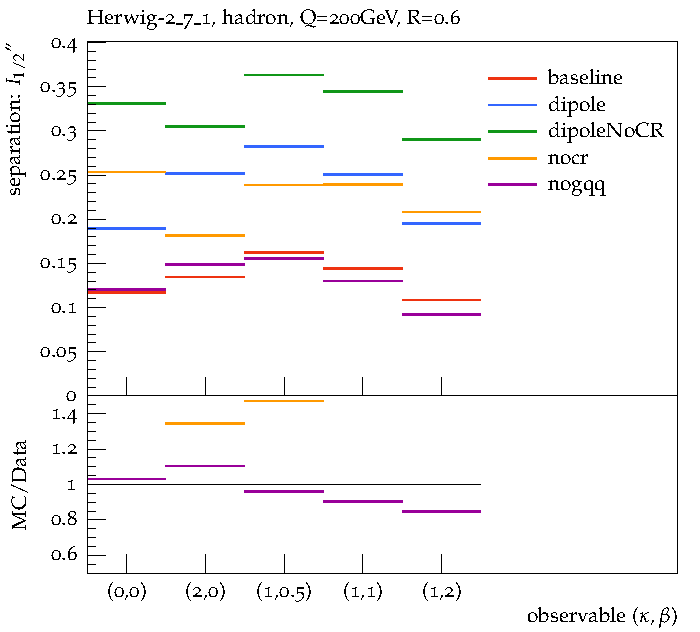
\includegraphics[width = 0.45\columnwidth]{quarkgluon_fig_I2_R6_hadron_herwig.pdf}
\label{quarkgluon_fig:summary_hadron_herwig}
}
$\qquad$
\subfloat[]{
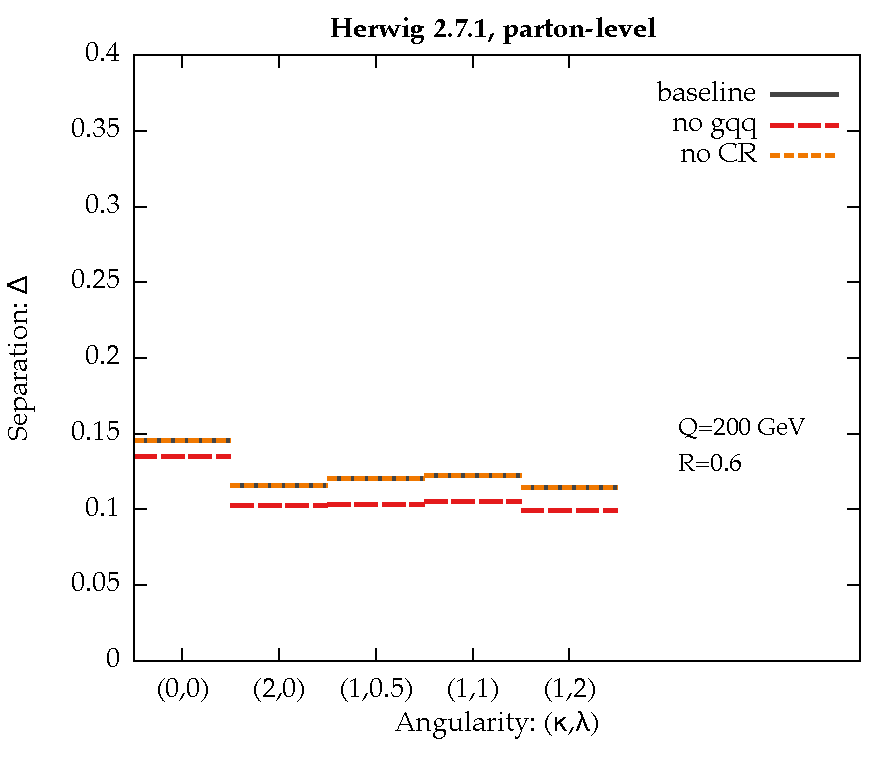
\includegraphics[width = 0.45\columnwidth]{quarkgluon_fig_I2_R6_parton_herwig.pdf}
\label{quarkgluon_fig:summary_parton_herwig}
}
\caption{Same as Fig.~\ref{quarkgluon_fig:settings_variation_pythia}, but for \textsc{Herwig 2.7.1}.}
\label{quarkgluon_fig:settings_variation_herwig}
\end{figure}

Our \textsc{Herwig++} baseline uses version 2.7.1, with improved modeling of underlying event~\cite{Gieseke:2012ft} and the most recent UE-EE-5-MRST tune~\cite{Seymour:2013qka}, which is able to describe the double-parton scattering cross section~\cite{Bahr:2013gkj} and underlying event data from $\sqrt{s} = 300$~GeV to $\sqrt{s} = 7$~TeV.  In Fig.~\ref{quarkgluon_fig:settings_variation_herwig}, we consider the following  \textsc{Herwig} variations:
\begin{itemize}
\item \textsc{Herwig: no $g \to q\bar{q}$}.  Turning off $g \to q \bar{q}$ splittings in \textsc{Herwig} has the reverse behavior as seen in \textsc{Pythia}, leading to slightly worse discrimination power, though the effect is modest.
\item \textsc{Herwig: no CR}.  The variation turns off color reconnections in \textsc{Herwig}.  This has no effect at parton level, as expected.  At hadron level, this variation for \textsc{Herwig} gives a rather dramatic improvement in quark/gluon discrimination power.  We think this arises since color reconnection in \textsc{Herwig} allows any color-anticolor pair to reconnect, even if they arose from an initially color octet configuration.  By turning off color reconnection, the gluons look more octet-like, explaining the improvement seen.
%\item \textsc{Herwig: Dipole}.  The default \textsc{Herwig} shower is based on angular ordering, but this variation uses a dipole shower instead.  Since this shower is closer in spirit to \textsc{Pythia}, one expects it to yield improved quark/gluon discrimination, which it does.
%\item \textsc{Herwig: Dipole, No CR}.  By switching to the dipole shower without color reconnections, one can make \textsc{Herwig} look rather similar to \textsc{Pythia} in terms of predicted discrimination performance.  Therefore, LHC data will be essential to understand which shower structure is closer to nature.
\end{itemize}
The importance of color reconnections in \textsc{Herwig} is a big surprise from this study, motivating future detailed studies into which color reconnection models are most realistic when compared to data.  In the future, we also plan to test the default angular-ordered \textsc{Herwig} shower against an alternative dipole shower \cite{Platzer:2011bc}.

\begin{figure}
\centering
\subfloat[]{
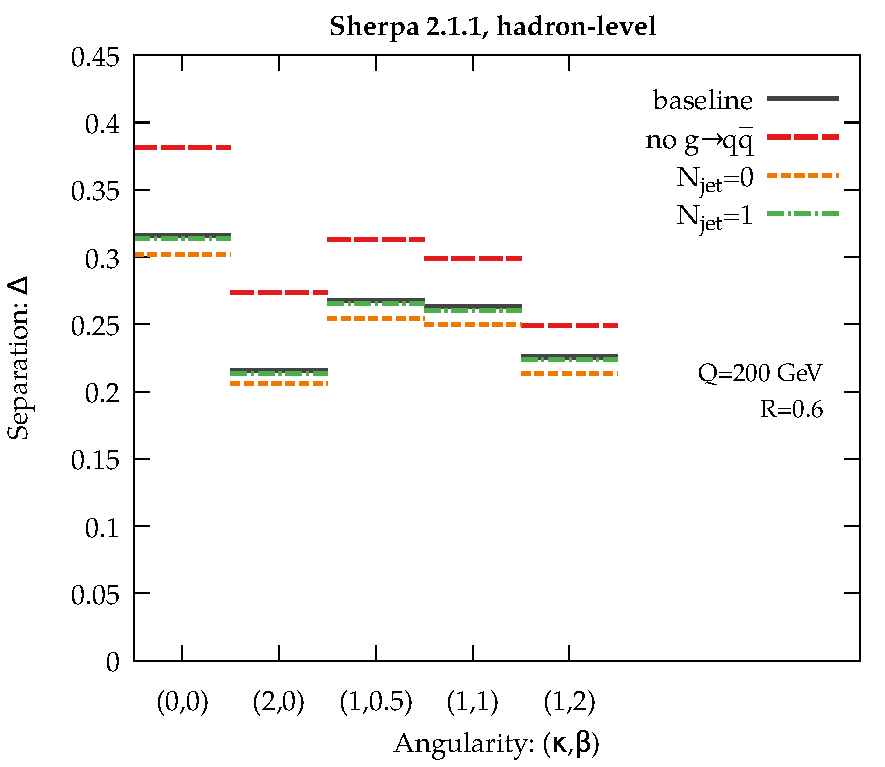
\includegraphics[width = 0.45\columnwidth]{quarkgluon_fig_I2_R6_hadron_sherpa.pdf}
\label{quarkgluon_fig:summary_hadron_sherpa}
}
$\qquad$
\subfloat[]{
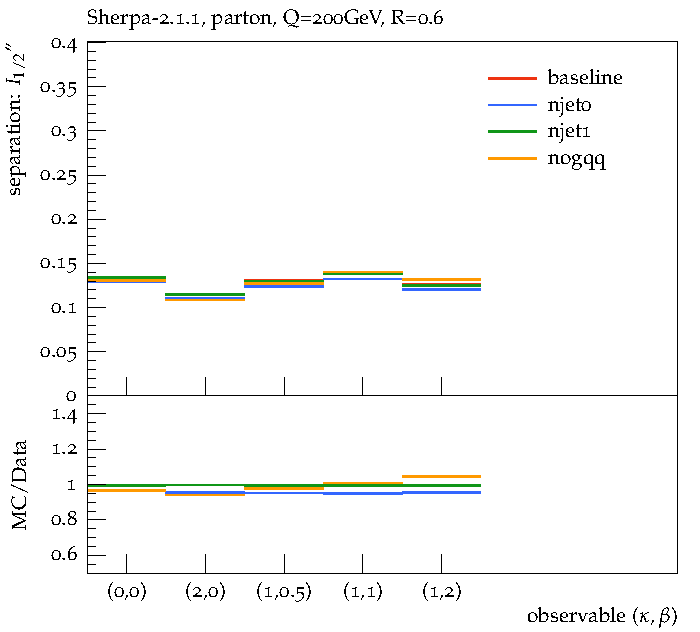
\includegraphics[width = 0.45\columnwidth]{quarkgluon_fig_I2_R6_parton_sherpa.pdf}
\label{quarkgluon_fig:summary_parton_sherpa}
}
\caption{Same as Fig.~\ref{quarkgluon_fig:settings_variation_pythia}, but for \textsc{Sherpa 2.1.1}.}
\label{quarkgluon_fig:settings_variation_sherpa}
\end{figure}

Our  \textsc{Sherpa} baseline uses matrix element corrections for the first two emissions ($N_\text{jet} = 2$) with CKKW-style matching \cite{Catani:2001cc}.  In Fig.~\ref{quarkgluon_fig:settings_variation_sherpa}, we consider the following \textsc{Sherpa} variations:
\begin{itemize}
\item \textsc{Sherpa: No $g \to q\bar{q}$}.  Turning off $g \to q \bar{q}$ splittings in \textsc{Sherpa} has a negligible effect at parton level, but it leads to a large jump in discrimination power at hadron level, again due to an interplay between the perturbative shower and nonperturbative hadronization.
\item \textsc{Sherpa: $N_\mathrm{jet} = 1$}.  This variation only performs CKKW matching for the first emission, leading to negligible changes in the discrimination performance.
\item \textsc{Sherpa: $N_\mathrm{jet} = 0$}.  Turning off all matrix element corrections in \textsc{Sherpa} slightly decreases the predicted quark/gluon discrimination power, in agreement with the behavior of \textsc{Pythia}.
\end{itemize}
Within \textsc{Sherpa}, matrix element corrections appear to have a very small effect at parton level.  The large changes seen at hadron level from turning off $g \to q \bar{q}$ splittings motivates further investigations into the shower/hadronization interface.

\begin{figure}
\centering
\subfloat[]{
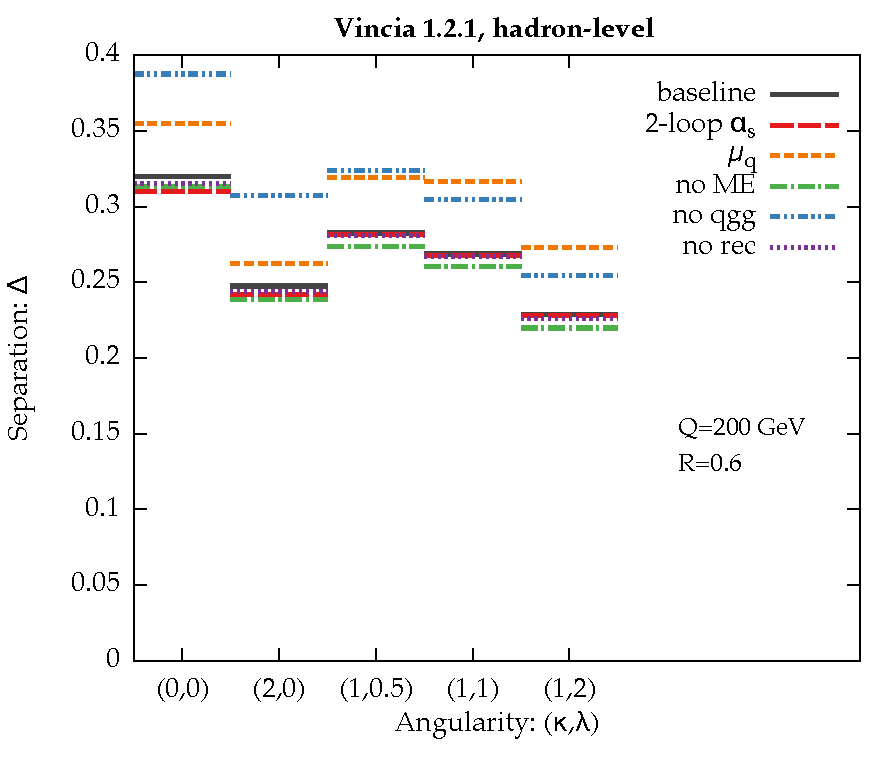
\includegraphics[width = 0.45\columnwidth]{quarkgluon_fig_I2_R6_hadron_vincia.pdf}
\label{quarkgluon_fig:summary_hadron_vincia}
}
$\qquad$
\subfloat[]{
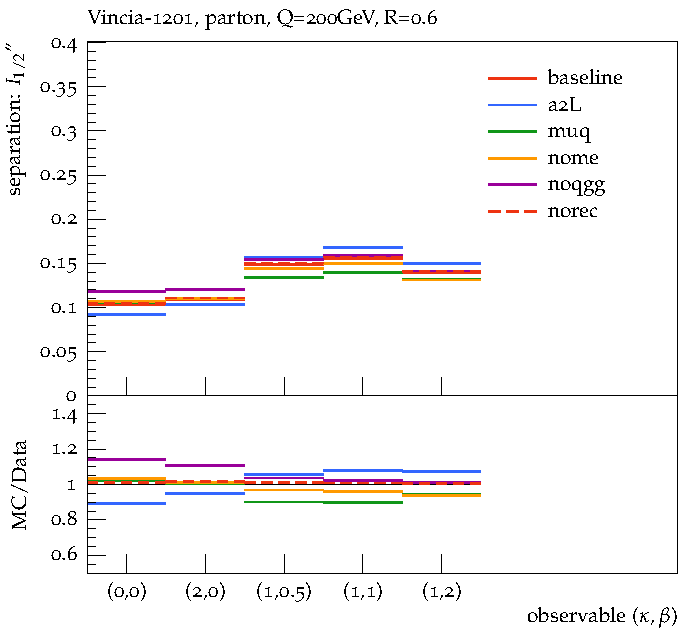
\includegraphics[width = 0.45\columnwidth]{quarkgluon_fig_I2_R6_parton_vincia.pdf}
\label{quarkgluon_fig:summary_parton_vincia}
}
\caption{Same as Fig.~\ref{quarkgluon_fig:settings_variation_pythia}, but for \textsc{Vincia 1.201}.}
\label{quarkgluon_fig:settings_variation_vincia}
\end{figure}

Our \textsc{Vincia} baseline is based on the ``jeppsson5'' tune.  While \textsc{Vincia} has NLO matrix elements for $e^+ e^- \to q \bar{q}$, it does not have them for $e^+ e^- \to gg$, so we will use LO \textsc{Vincia} throughout.  In Fig.~\ref{quarkgluon_fig:settings_variation_vincia}, we consider the following \textsc{Vincia} variations:
\begin{itemize}
\item \textsc{Vincia:  no $g \to q\bar{q}$}.  This variation turns off $g \to q \bar{q}$, leading to the expected increase in separation power as seen in \textsc{Pythia}.
\item \textsc{Vincia: no ME}.  By default, each $2 \to 3$ antenna in \textsc{Vincia} has an associated matrix element correction factor.  Since the antenna are already rather close to the true matrix elements, turning off these matrix elements has a modest effect on quark/gluon discrimination power.
\item \textsc{Vincia: 2-loop $\alpha_s$}.  Like for \textsc{Pythia}, this variation switches from 1-loop to 2-loop $\alpha_s$ running, yielding a modest parton-level difference and almost no hadron-level difference. 
\item \textsc{Vincia: alt $\mu_q$}.  By default, the $\alpha_s$ scale used in \textsc{Vincia} is determined by the transverse momentum of the corresponding antenna.  In this variation, the $\alpha_s$ scale is set to half the invariant mass of the mother antenna.  This slightly decreases the discrimination power at hadron level, but increases the discrimination power at parton level, again showing the complicated interplay of perturbative and nonperturbative effects.
\end{itemize}
Since \textsc{Vincia} and \textsc{Pythia} share the same underlying engine, it is not surprising that they exhibit similar behaviors as parameters are changed.  The biggest surprise is the way that changing the $\alpha_s$ scale for the antenna can lead to different trends at parton and hadron level.

Our \textsc{Deductor} baseline uses leading color plus (LC+) showering, which includes some subleading color structures. We find that switching from LC+ to LC showering at parton level has a negligible impact on quark/gluon discrimination power.  When \textsc{Deductor} interfaces with the default tune of \textsc{Pythia 8.212} for hadronization, only leading color is used in the showering, such that partons with their LC color information can be directly passed to the Lund string model.  No \textsc{Deductor} variations are shown here, but we anticipate studying the effect of $g \to q \bar{q}$ splitting in future work.

\begin{figure}
\centering
\subfloat[]{
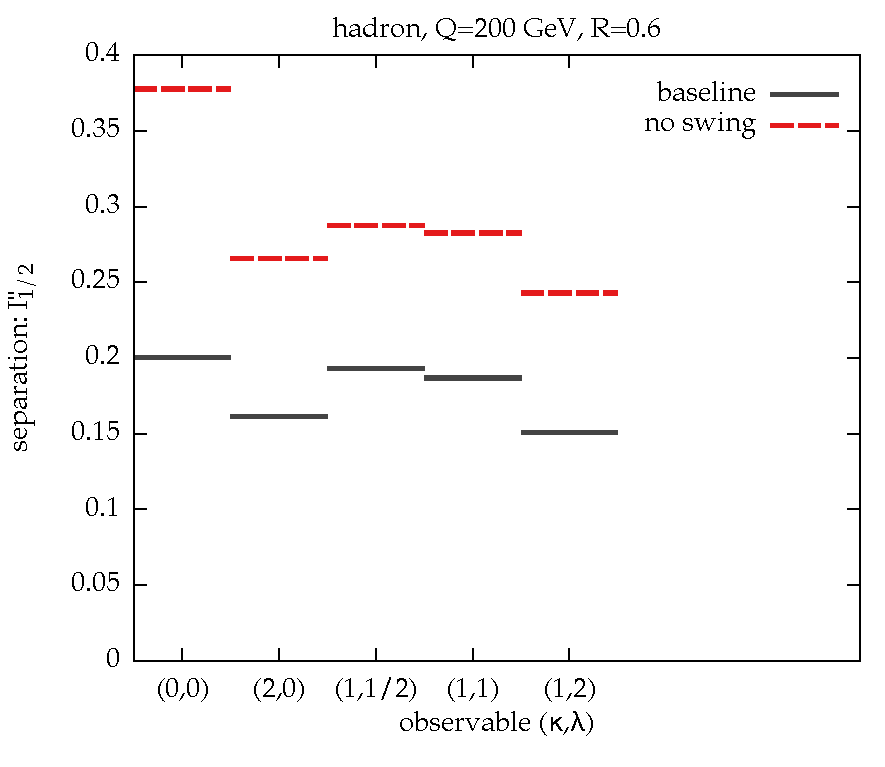
\includegraphics[width = 0.45\columnwidth]{quarkgluon_fig_I2_R6_hadron_ariadne.pdf}
\label{quarkgluon_fig:summary_hadron_ariadne}
}
$\qquad$
\subfloat[]{
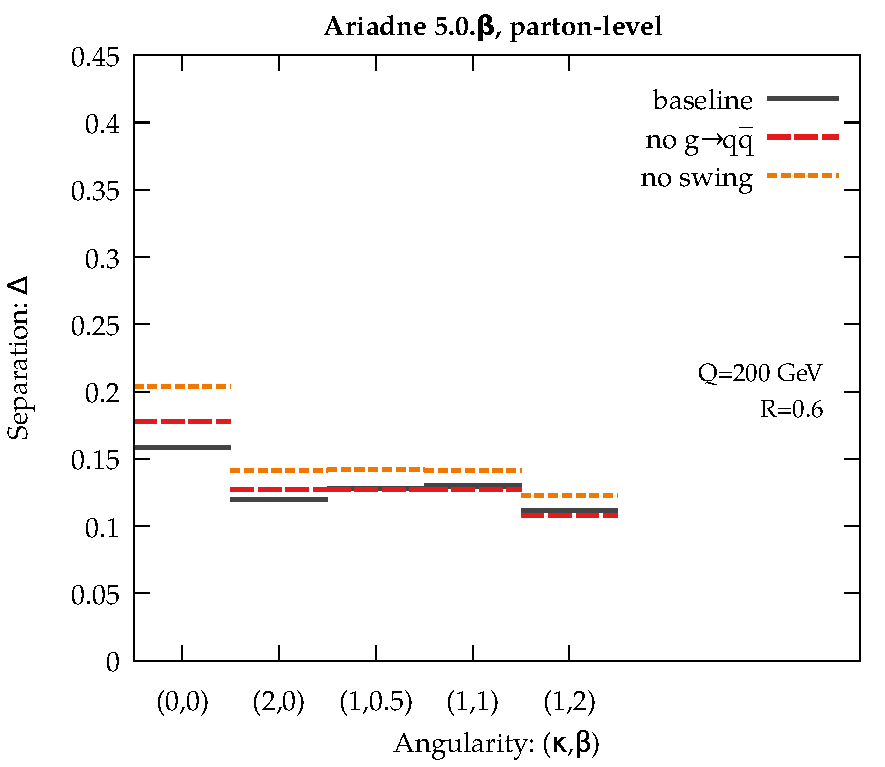
\includegraphics[width = 0.45\columnwidth]{quarkgluon_fig_I2_R6_parton_ariadne.pdf}
\label{quarkgluon_fig:summary_parton_adriadne}
}
\caption{Same as Fig.~\ref{quarkgluon_fig:settings_variation_pythia}, but for \textsc{Ariadne 5.0.$\beta$}.}
\label{quarkgluon_fig:settings_variation_ariadne}
\end{figure}

Finally, our \textsc{Ariadne} baseline is based on a beta release of version 5.  In Fig.~\ref{quarkgluon_fig:settings_variation_ariadne}, we consider the following \textsc{Ariadne} variation:
\begin{itemize}
\item \textsc{Ariadne:  no $g \to q\bar{q}$}.  This variation turns off $g \to q \bar{q}$, leading to modest change in separation power, similar in magnitude to \textsc{Herwig}.
\item \textsc{Ariadne: no swing}.  Swing refers to color reconnections performed during the perturbative cascade, where dipoles in the same color state are allowed to reconnect in a way which prefers low-mass dipoles  \cite{Flensburg:2011kk,Bierlich:2014xba}.  Turning off swing has an effect already at parton level, which is amplified at hadron level, leading to improved quark/gluon separation.
\end{itemize}
Like for \textsc{Pythia} and \textsc{Herwig}, color reconnections play a surprisingly important role in \textsc{Ariadne}.

\subsection{Looking Towards the LHC}
\label{quarkgluon_sec:pp}

It is clear from our $e^+e^-$ study that quark/gluon radiation patterns face considerable theoretical uncertainties, as seen from the differing behaviors of parton shower generators.  This is true even accounting only for final state physics effects, so additional initial state complications can only increase the uncertainties faced in $pp$ collisions.  Beyond just the application to quark/gluon tagging, this is an important challenge for any analysis that uses jets.  For example, a proper experimental determination of jet energy scale corrections requires robust parton shower tools that correctly model effects like out-of-cone radiation.  Eventually, one would like to perform improved analytic calculations to address these radiation pattern uncertainties.  In the near term, though, measurements from the LHC will be essential for improving the parton shower modeling of jets.

\begin{figure}
\centering
\subfloat{
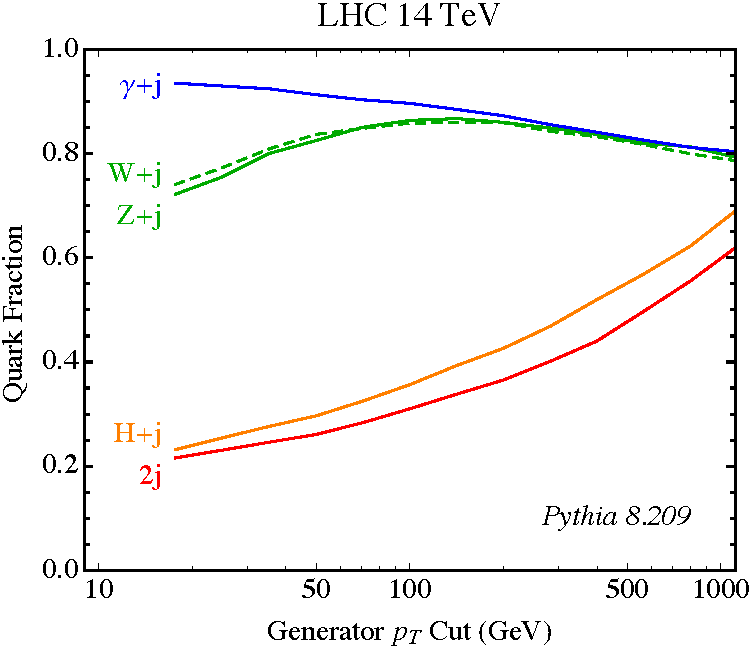
\includegraphics[width = 0.45\columnwidth]{quarkgluon_fig_parton_level_qg_composition.pdf}
}
\caption{Quark fraction of jets at parton level, as defined by the Born-level parton flavor.}
\label{quarkgluon_fig:parton_level_qg_composition}
\end{figure}

At the LHC, there is no way to isolate pure samples of quark or gluon jets, but one can isolate quark/gluon-enriched samples, as defined by the flavor label of the jet in the corresponding Born-level partonic process.  As shown in Fig.~\ref{quarkgluon_fig:parton_level_qg_composition}, the Born-level jet in $W/Z/\gamma + \text{jet}$ is more than 70\% quark enriched over the entire jet $p_T$ range of interest.  For jets softer than around 200 GeV, the Born-level jet in dijets or $H+\text{jet}$ is more than 60\% gluon enriched, with that fraction decreasing as the jet $p_T$ increases.  More sophisticated enrichment procedures are described in Ref.~\cite{Gallicchio:2011xc}.

In principle, one could try to ``diagonalize" some combination of vector boson plus jet and dijet samples in order to define separate quark or gluon samples (see e.g.~\cite{Aad:2014gea}).  In the spirit of Sec.~\ref{quarkgluon_sec:def}, though, we think it is more beneficial for the LHC experiments to perform process-specific measurements without trying to directly determine their quark and gluon composition.  For example, instead of quark/gluon separation, one can ask the more well-defined question about whether one can tell ``the jet in $Z$ plus jets" (quark-enriched) apart from ``the jet in dijets" (gluon-enriched).  Similarly, one could test for differences within a jet sample, such as comparing central jets versus forward jets in dijet production.  This process-based strategy is also helpful for sidestepping the known process dependance of defining quarks and gluons at the LHC, where color correlations to the rest of the event impede a universal definition of quark and gluon jets.

Already, one would learn a lot from unfolded measurements at the LHC  of the generalized angularities in a variety of quark/gluon enriched samples.  Even detector-level measurement comparing a wide range of generators (and generator modifications) would help in understanding how to improve quark/gluon modeling.   The five benchmark angularities in Eq.~\eqref{quarkgluon_eq:benchmarkang} probe both the perturbative and nonperturbative structure of jets and are therefore a good starting point for a more comprehensive quark/gluon jet shape analysis.  In this spirit, we are encouraged by the track multiplicity study of Ref.~\cite{Aad:2016oit}, though for parton shower tuning is it is important to have measurements not only of jet shape averages but also of the full jet shape probability distributions.

Finally, we think it would be useful to perform LHC jet shape measurements after jet grooming (see e.g.~\cite{Butterworth:2008iy,Ellis:2009su,Ellis:2009me,Krohn:2009th}).  Often jet grooming is described as a pileup mitigation strategy, but even independent of pileup, grooming modifies the observed jet radiation patterns in ways that are interesting from the quark/gluon perspective.  Using techniques from Refs.~\cite{Dasgupta:2013ihk,Larkoski:2014wba}, one can calculate the quark/gluon discrimination power for angularities after jet grooming.  Those calculations generically predict that groomed jet shapes should have reduced quark/gluon discrimination power compared to ungroomed jet shapes.  That said, because techniques like soft drop \cite{Larkoski:2014wba} remove soft radiation from jets, they tend to reduce the process dependence in quark/gluon radiation patterns, and may therefore yield a more robust theoretical definition for quark and gluon jets.

\subsection{Summary and Recommendations}
\label{quarkgluon_sec:conclude}

By measuring the substructure of jets, one can gain valuable information about the quark/gluon composition of a jet sample.  The challenge we have identified in this study is that the precise radiation patterns of quark and gluon jets is poorly understood, in the sense that parton shower generators give rather different predictions for absolute quark/gluon discrimination power as well as relative trends as a function of the jet kinematics.  At the moment, analytic calculations are not at a level of accuracy where they can offer a useful guide.  Therefore, LHC measurements are the best near-term strategy to constrain quark/gluon radiation patterns and enable quark/gluon discrimination to become a robust experimental tool.

In terms of specific measurements that should be highest priority for ATLAS and CMS, our study has not revealed a silver bullet.  Rather, all of the generalized angularities studied here showed similar levels of disagreement between generators, so a systematic LHC study of even one observable is likely to offer crucial new information.  What is essential is to make measurements at multiple jet $p_T$ scales with multiple jet radii $R$ in multiple different jet samples.  Unfolded distributions would be most useful for parton shower tuning, but even detector-level measurements compared to detector-simulated parton showers would help spot troubling trends.  For the IRC safe angularities in particular, studying the $\beta$ dependence would help separate information about collinear and soft radiation patterns, especially given the fact that the $\beta$ trends seen in the parton shower generators here disagree with those seen in Ref.~\cite{Aad:2014gea}.

If possible, it would be interesting to study the LHA ($\beta = 1/2$) on archival LEP data, since this angularity probes the core of jets in a new way, distinct from broadening-like ($\beta = 1$) or thrust-like ($\beta = 2$) observables.  Among the IRC safe angularities studied here, LHA has the best predicted discrimination power, making it (and other $0<\beta < 1$ angularities) a well-motivated target for future lepton collider measurements.  Similarly, it would be worthwhile to improve our analytic understanding of the LHA.  From Fig.~\ref{quarkgluon_fig:LHA_hadron_separation}, we see that the LHA has discrimination power both at small values of $\lambda_{0.5}^1$ (where non-perturbative corrections play an important role) as well as at larger values of $\lambda_{0.5}^1$ (where fixed-order corrections are important), so one must go beyond an NLL understanding to understand the quark/gluon performance of the LHA.


The key lesson to parton shower authors is that, contrary to some standard lore, existing LEP measurements \emph{do not} constrain all of the relevant aspects of the final state parton shower.  While we have extensive information about quark jet radiation patterns from LEP event shapes, gluon jet radiation patterns are largely unconstrained.  This has important implications for parton shower tuning strategies, since LHC data can and should be used to adjust final state shower parameters.  For example, the ATLAS A14 tune of \textsc{Pythia} has a 10\% lower value of $\alpha_s$ in the final state shower compared to the Monash tune, which yields better agreement with charge particle multiplicity distributions \cite{Aad:2016oit}.  However, A14 has not been tested on LEP event shapes, suggesting that a global tuning strategy is needed.   In addition, it is worth mentioning that similar quark/gluon studies have been carried out in deep inelastic electron-proton scattering \cite{Chekanov:2004kz}, which offer an intermediate step between $pp$ and $e^+ e^-$ collisions, and this $ep$ data could also be valuable for parton shower tuning.

Based on this study, we have identified three aspects of the final state parton shower that deserve closer scrutiny.
\begin{itemize}
\item \textit{Gluon splitting to quarks}.  Some of the largest differences between generators came from turning on and off the $g \to q \overline{q}$ splitting process.  While \textsc{Pythia}, \textsc{Sherpa}, \textsc{Vincia}, and \textsc{Ariadne} suggest that (unphysically) turning off $g \to q \overline{q}$ would improve quark/gluon separation, \textsc{Herwig} (and the analytic calculation in Ref.~\cite{Larkoski:2013eya}) suggests the opposite conclusion.  Beyond quark/gluon discrimination, it would be helpful to identify other contexts where $g \to q \overline{q}$ might play an important role.
\item \textit{Color reconnection in the final state}.  Color reconnection is often thought of as an issue mainly at hadron colliders, but we have seen that it can have an impact in $e^+ e^-$ collisions as well.  This is particularly the case with the default color reconnection model in \textsc{Herwig}, since it allows the reconnection of color/anticolor lines even if they originally came from an octet configuration.  We also saw large changes from \textsc{Pythia: CR1} and  \textsc{Ariadne: no swing}, suggesting that one should revisit color reconnection physics when tuning to LEP data.
\item \textit{Reconsidering $\alpha_s$ defaults}:  In the context of parton shower tuning, the value of $\alpha_s$ used internally within a code need not match the world average value, since higher-order effects not captured by the shower can often be mimicked by adjusting $\alpha_s$.  That said, one has to be careful whether a value of $\alpha_s$ tuned for one process is really appropriate for another.  For example, \textsc{Pythia} uses a relatively large value of $\alpha_s$ in its final state shower, which allows it to match LEP event shape data.  The same value of $\alpha_s$, though, probably also leads to too much radiation within gluon jets.
\end{itemize}
Finally, we want to emphasize that despite the uncertainties currently present in parton shower generators, parton showers in particular (and QCD resummation techniques more generally) will be essential for understanding quark/gluon discrimination.  Fixed-order QCD calculations cannot reliably probe the very soft and very collinear structure of jets, which is precisely where valuable information about quark/gluon radiation patterns reside.  Given the ubiquity and value of parton shower generators, improving the understanding of quark/gluon discrimination will assist every jet study at the LHC.

\subsection*{Acknowledgments}

DK acknowledges support from the Science Faculty Research Council, University of Witwatersrand.
%
The work of LL, SP, and AS is supported in part by the MCnetITN FP7 Marie Curie Initial Training Network, contract PITN-GA-2012-315877.
%
LL is also support by the Swedish Research Council (contracts 621-2012-2283 and 621-2013-4287).
%
SP acknowledges support from a FP7 Marie Curie Intra European Fellowship under Grant Agreement PIEF-GA-2013-628739.
%
The work of DS is supported by the U.S. Department of Energy (DOE) under Grant DE-SC-0011640.
%
The work of GS is supported by the Paris-Saclay IDEX under the IDEOPTIMALJE grant. 
%
The work of JT is supported by the DOE under cooperative research agreement DE-SC-00012567, by the DOE Early Career research program DE-SC-0006389, and by a Sloan Research Fellowship from the Alfred P. Sloan Foundation.

\bibliography{quarkgluon_bib}

\end{document}
